\documentclass[preprint,3p,times]{elsarticle}

\usepackage{amsmath,amssymb}
\usepackage{graphicx}
\usepackage{booktabs}
\usepackage{multirow}
\usepackage{algorithm}
\usepackage{algorithmic}
\usepackage{hyperref}
\usepackage{geometry}

\journal{Acta Astronautica}

\graphicspath{{./figures/}}

\begin{document}

\begin{frontmatter}

\title{Simultaneous Estimation and Control via a Common State-Dependent Coefficient Matrix for Angles-Only Relative Navigation in Elliptical Orbits}

\author[1]{First Author}
\author[1]{Second Author}
\address[1]{Institution, City, Country}

\begin{abstract}
This paper presents a comprehensive closed-loop validation of a common State-Dependent Coefficient (SDC) parameterization for angles-only relative navigation in elliptical orbits, where a single $A_{\text{SDC}}(t_k)$ matrix simultaneously drives the extended Kalman filter (EKF) prediction step and the state-dependent Riccati equation (SDRE) optimal control computation. Because the SDC parameterization satisfies the algebraic identity $A(x) \cdot x \equiv f(x)$, the EKF linearization point $\hat{x}_{k|k}$ and the controller design point share the same state-dependent system matrix---eliminating the model mismatch that arises when estimation and control use different dynamical representations. A forward-Euler SDC discretization introduces a median per-step position error of 1.15~m, two orders of magnitude below the angles-only measurement uncertainty (${\sim}140$~m at typical ranges), confirming that the common-matrix discretization is numerically adequate for closed-loop purposes.

Closed-loop performance is evaluated on a medium-Earth orbit scenario ($a_c = 15{,}000$~km, $e_c = 0.5$, initial separation 866~km) through five experiment groups: (A)~angles-only EKF+SDRE versus full-information SDRE, (B)~sensor noise sensitivity sweep ($\sigma_\theta \in [0.001^\circ, 0.1^\circ]$, 30 trials), (C)~CW linear model baseline on NERM truth dynamics ($e \in [0.001, 0.7]$), (D)~orbital regime sensitivity (LEO, MEO, GEO), and (E)~a 200-trial Monte Carlo analysis with randomized initial conditions. The angles-only EKF+SDRE first crosses the 100-m approach threshold at 54,800~s with a position RMSE of 8.16~km. Increasing sensor noise from $0.001^\circ$ to $0.1^\circ$ shortens this first-passage time by a factor of 2.3 (87,000~s to 38,220~s) while peak thrust and total $\Delta V$ remain nearly constant; however, terminal relative velocity increases by approximately 20$\times$, and configurations with $\sigma_\theta > 0.004^\circ$ fail a tightened soft-arrival criterion. This behavior is therefore a speed--softness trade-off under a distance-only stopping condition, not an improvement in rendezvous quality. The CW model diverges at all tested eccentricities---the root cause is an 80\% overestimation of the gravity gradient at 866~km, not orbital eccentricity. Monte Carlo analysis yields a 97.5\% distance-threshold success rate (195/200, 95\% CI: [94.3\%, 99.1\%]) with a median first-passage time of 13.4~h. These results show that while the common SDC-matrix approach is reliable for threshold-reaching tasks in the tested MEO regime, its validity is bounded: LEO operations fail due to Coriolis-induced control authority saturation, GEO operations are susceptible to stochastic EKF divergence from innovation wrapping under frozen Kalman gains, and terminal rendezvous requires an explicit velocity-constrained guidance phase.
\end{abstract}

\begin{keyword}
angles-only navigation \sep extended Kalman filter \sep state-dependent Riccati equation \sep spacecraft relative motion \sep relative navigation \sep elliptical orbit
\end{keyword}

\end{frontmatter}

%=====================================================================
\section{Introduction}
%=====================================================================

\subsection{Problem Context}

Spacecraft relative navigation and autonomous approach are fundamental capabilities for on-orbit servicing, debris removal, formation flying, and non-cooperative target proximity operations. These missions require the chaser spacecraft to estimate the relative position and velocity of a target using onboard sensors, and to compute control commands that reduce the relative distance to enable docking, capture, or inspection.

Optical cameras represent the most practical onboard sensor for relative navigation, providing bearing measurements (azimuth and elevation angles) but no direct range information. This angles-only measurement constraint introduces a fundamental observability challenge: under linear constant-velocity dynamics, relative range cannot be uniquely determined from angular measurements alone~\cite{Woffinden2009}.

A second challenge arises from the orbital environment: spacecraft operating in elliptical orbits experience time-varying and nonlinear gravitational effects that violate the assumptions of the classical Clohessy-Wiltshire (CW) linear model~\cite{Clohessy1960}. While the CW equations assume a circular reference orbit and small separations, real mission scenarios frequently involve elliptical orbits with separations of hundreds to thousands of kilometers, where nonlinear gravitational differential effects become non-negligible.

A third challenge is methodological: the estimation and control subsystems in a relative navigation architecture typically employ different dynamical models---for instance, a linearized CW model for the EKF and a nonlinear model for the controller. This model mismatch can degrade both estimation accuracy and control performance, yet it is rarely addressed systematically.

\subsection{Related Work}

\textbf{Relative motion dynamics.} The CW equations~\cite{Clohessy1960} provide a closed-form linear model for relative motion under a circular chief orbit assumption. The Tschauner-Hempel (TH) equations~\cite{Tschauner1965} extend the linearization to elliptical orbits but introduce time-varying periodic coefficients. Yamanaka and Ankersen~\cite{Yamanaka2002} derived a nonsingular state transition matrix for the TH equations. However, linearizations of the gravitational potential assume $|\boldsymbol{\rho}| \ll |r_c|$, which breaks down at large separations. Karlgaard and Lutze~\cite{Karlgaard2003} quantified the second-order nonlinear corrections to CW that become non-negligible beyond a few tens of kilometers. For long-range relative navigation in elliptical orbits, full nonlinear models become necessary~\cite{Dwidar2013}. Alfriend et al.~\cite{Alfriend2009} provide a comprehensive treatment of spacecraft formation flying dynamics spanning linear, nonlinear, and perturbed models.

\textbf{Angles-only relative navigation.} Woffinden and Geller~\cite{Woffinden2009,Woffinden2009b} established the fundamental observability criteria for angles-only navigation, proving that under linear CW dynamics, relative state is not fully observable from angular measurements alone, and subsequently characterized optimal rendezvous maneuvers that enhance observability. Geller and Klein~\cite{Geller2014} showed that a camera offset from the center of mass can restore observability without propulsive maneuvers. Gaias, D'Amico, and Ardaens~\cite{Gaias2014} demonstrated angles-only relative navigation using relative orbital elements (ROE) on the PRISMA and AVANTI flight experiments, confirming that state parameterizations tailored to orbital geometry can mitigate nonlinear estimation challenges under perturbed dynamics. Sullivan and D'Amico~\cite{Sullivan2017} applied nonlinear Kalman filtering with ROE for improved angles-only estimation; the same authors later generalized the architecture to distributed multi-satellite formations~\cite{Sullivan2021}. The use of ROE provides slow-varying states that simplify relative navigation under J2 perturbations, highlighting the utility of geometric state design.

\textbf{SDRE optimal control.} The State-Dependent Riccati Equation method, introduced by Cloutier~\cite{Cloutier1997} and comprehensively surveyed by \c{C}imen~\cite{Cimen2012,Cimen2010}, extends linear quadratic optimal control to nonlinear systems through SDC parameterization. The key insight is that a nonlinear system $\dot{x} = f(x)$ can be factorized as $\dot{x} = A(x)x + B(x)u$, enabling pointwise solution of an algebraic Riccati equation to obtain a nonlinear feedback law. The SDRE approach has been applied to spacecraft formation flying~\cite{Dwidar2013}, rendezvous~\cite{Tartaglia2016}, and proximity operations.

\textbf{SDRE filtering (SDREF).} Mracek, Cloutier, and D'Souza~\cite{Mracek1996} extended the SDRE concept to nonlinear estimation, proposing the SDREF as an alternative to the EKF. Park and Kim~\cite{Park2016} applied SDREF to spacecraft formation flying relative navigation, demonstrating that SDREF achieves the computational speed of linearized EKF with the accuracy of numerically integrated EKF (3-D RMS position 6.0~mm at 50~km separation). Simhamed and Ykhlef~\cite{Simhamed2021} benchmarked SDREF against EKF and found superior noise robustness and accuracy.

\textbf{Estimation-control integration.} Vepa~\cite{Vepa2018} combined nonlinear TH equations with estimation and control using an LQNG methodology. Okasha and Newman~\cite{Okasha2011} used a TH-based EKF with glideslope guidance for autonomous rendezvous. Choukroun and Tekinalp~\cite{Choukroun2013} applied SDRE to both the estimation and control of spacecraft \emph{attitude}, demonstrating that the SDRE method can serve dual roles---this is conceptually the closest prior work, though in a different dynamical domain (attitude rather than relative position). Lee, Cochran, and No~\cite{Lee2012} combined an SDRE controller with an EKF for spacecraft formation flying, but employed different dynamical models for the two subsystems. Muralidhar and Kumar~\cite{Muralidhar2021} used an SDRE controller with a UKF estimator based on TH equations for elliptical-orbit rendezvous and docking.

\begin{table}[h]
\centering
\caption{Relationship between the present work and closely related prior studies.}
\label{tab:prior_work}
\begin{tabular}{lcccc}
\toprule
Study & Domain & Filter & Controller & Common $A_{\text{SDC}}$? \\
\midrule
Park \& Kim~\cite{Park2016} & Rel.\ position & SDREF & --- (estimation only) & N/A \\
Choukroun \& Tekinalp~\cite{Choukroun2013} & Attitude & SDREF & SDRE & Yes (same domain) \\
Lee et al.~\cite{Lee2012} & Rel.\ position & EKF (linearized) & SDRE & No \\
Muralidhar \& Kumar~\cite{Muralidhar2021} & Rel.\ position & UKF (TH-based) & SDRE & No \\
\textbf{This work} & \textbf{Rel.\ position} & \textbf{EKF (SDC-based)} & \textbf{SDRE} & \textbf{Yes} \\
\bottomrule
\end{tabular}
\end{table}

The key architectural distinction is that in the present work, the identical SDC matrix $A_{\text{SDC}}(\hat{x}_{k|k})$ evaluated at the EKF state estimate is used directly for both prediction and control---the estimation and control subsystems share not only the same dynamical model \emph{class} but the same numerical matrix instance at each time step. Park and Kim~\cite{Park2016} validated SDREF for relative navigation but did not close the loop with SDRE control. Choukroun and Tekinalp~\cite{Choukroun2013} used SDRE for both estimation and control but in the attitude domain, where the dynamics and measurement structure differ fundamentally from relative position navigation. Lee et al.~\cite{Lee2012} and Muralidhar and Kumar~\cite{Muralidhar2021} each used different dynamical representations for the filter and the controller.

\subsection{Research Gap and Contributions}

An underexplored opportunity exists at the intersection of these domains. SDREF employs an SDC parameterization for filtering~\cite{Park2016}, and SDRE has been extensively applied to control~\cite{Cimen2012}. Since the SDC representation satisfies the algebraic identity $A(x)\cdot x \equiv f(x)$, the same state-dependent matrix evaluated at the filter estimate $\hat{x}_{k|k}$ can, in principle, serve both subsystems---eliminating the model mismatch that arises when estimation and control employ different dynamical models. However, the closed-loop performance and limitations of such a common-parameterization architecture for \emph{relative position} navigation under angles-only constraints have not been systematically characterized. Table~\ref{tab:prior_work} summarizes the relationship between the present work and the most closely related prior studies.

This paper presents a comprehensive experimental validation and characterization of the common SDC-matrix approach, making the following contributions:

\begin{enumerate}
    \item \textbf{Comprehensive closed-loop validation of the common SDC-matrix architecture.} We present a five-experiment characterization of angles-only EKF estimation supporting SDRE optimal approach control in elliptical orbits: baseline comparison, sensor noise sensitivity, CW model baseline, orbital regime sensitivity, and a 200-trial Monte Carlo analysis yielding a 97.5\% distance-threshold success rate (195/200, 95\% CI: [94.3\%, 99.1\%]). We show that while the method is reliable for threshold-reaching tasks in MEO, it fails under nominal parameters in LEO due to Coriolis control saturation and in GEO due to covariance freezing, defining the physical boundaries of the tested co-design.

    \item \textbf{Quantitative justification of the common-matrix discretization.} A diagnostic experiment comparing forward-Euler SDC discretization against fourth-order Runge-Kutta integration of the full nonlinear relative dynamics shows a median per-step position difference of only 1.15~m---two orders of magnitude below the angles-only measurement uncertainty, establishing numerical adequacy for closed-loop purposes.

    \item \textbf{Systematic failure analysis of the CW linear model.} We show that the CW model fails on NERM truth dynamics at \emph{all} tested eccentricities ($e \in [0.001, 0.7]$). The failure mechanism is identified as an 80\% overestimation of the gravity gradient at 866~km separation combined with the absence of NERM's nonlinear anti-damping modes---establishing that NERM-based dynamics are a \emph{necessity} for medium-to-long-range relative navigation, regardless of orbital eccentricity.

    \item \textbf{Characterization of a counterintuitive speed--softness trade-off.} We show that increasing sensor noise shortens the first-passage time through the 100-m approach sphere by a factor of 2.3 while peak thrust and total $\Delta V$ remain essentially constant, but terminal relative velocity increases by approximately 20$\times$. A tightened capture criterion demonstrates that the apparent acceleration is dominated by distance-threshold first passage rather than improved soft-rendezvous performance. A complementary true-state-$A_{\text{SDC}}$ ablation finds negligible direct coupling through the SDC linearization point for the tested single-seed MEO baseline, preventing that pathway from being overstated.

    \item \textbf{Engineering enhancements.} Symplectic balancing for ill-conditioned AREs (stabilizing matrices with $\|Q\|/\|S\| \approx 10^{13}$ condition number disparity) and sparse ARE update strategies are documented as practical contributions.
\end{enumerate}

The remainder of this paper is organized as follows. Section 2 describes the reference orbit dynamics, relative motion in the LVLH frame, and SDC parameterization. Section 3 presents the unified SDC matrix framework, including EKF prediction and SDRE control formulations. Section 4 outlines the simulation scenario, filter configurations, and experimental setup. Section 5 presents the numerical results, sensitivity analyses, and a comprehensive discussion of our findings. Finally, Section 6 concludes the paper and outlines directions for future work.

%=====================================================================
\section{System Modeling and Problem Formulation}
%=====================================================================

\subsection{Reference Orbit Dynamics}

We consider a chief spacecraft in a Keplerian elliptical orbit about the Earth, characterized by semi-major axis $a_c$, eccentricity $e_c$, and gravitational parameter $\mu = 3.986 \times 10^5~\text{km}^3/\text{s}^2$. The orbital motion is parameterized by the true anomaly $\nu$, which evolves according to:

\begin{align}
r_c(\nu) &= \frac{a_c(1 - e_c^2)}{1 + e_c \cos \nu} \label{eq:rc} \\
\dot{\nu} &= \frac{\sqrt{\mu a_c (1 - e_c^2)}}{r_c^2} \label{eq:nudot} \\
\ddot{\nu} &= -\frac{2 \dot{r}_c \dot{\nu}}{r_c}, \quad \dot{r}_c = \sqrt{\frac{\mu}{a_c(1-e_c^2)}}\, e_c \sin \nu \label{eq:nuddot}
\end{align}

\subsection{Nonlinear Relative Motion in the LVLH Frame}

The Local-Vertical Local-Horizontal (LVLH) frame is centered on the chief spacecraft: the $x$-axis points radially outward from Earth, the $z$-axis is aligned with the orbit normal, and the $y$-axis completes the right-handed triad (along-track direction).

The absolute states of the chaser (c) and target (t) are expressed in the LVLH frame as:
\begin{equation}
\mathbf{X}_c = [x_c, y_c, z_c, v_{xc}, v_{yc}, v_{zc}]^T, \quad
\mathbf{X}_t = [x_t, y_t, z_t, v_{xt}, v_{yt}, v_{zt}]^T
\end{equation}

The full system state is a 13-dimensional vector $\boldsymbol{\xi} = [\mathbf{X}_c^T, \mathbf{X}_t^T, \nu]^T$. The chaser's acceleration in the LVLH frame is:

\begin{align}
\ddot{x}_c &= 2\dot{\nu}\dot{y}_c + \ddot{\nu}y_c + \dot{\nu}^2 x_c - \frac{\mu(r_c + x_c)}{r_c^3} + \frac{\mu}{r_c^2} + u_{cx} \label{eq:accel_c} \\
\ddot{y}_c &= -2\dot{\nu}\dot{x}_c - \ddot{\nu}x_c + \dot{\nu}^2 y_c - \frac{\mu y_c}{r_c^3} + u_{cy} \\
\ddot{z}_c &= -\frac{\mu z_c}{r_c^3} + u_{cz}
\end{align}

where $r_c^{\text{geo}} = \sqrt{(r_c + x_c)^2 + y_c^2 + z_c^2}$ is the chaser's geocentric distance. The target's acceleration $\ddot{\mathbf{r}}_t$ follows the identical form with subscripts $t$, possibly including unknown maneuver accelerations $\mathbf{u}_t$ (treated as process noise or a disturbance by the chaser's filter). The differential control acceleration is $\mathbf{u} = [u_{cx}-u_{tx}, u_{cy}-u_{ty}, u_{cz}-u_{tz}]^T$.

\begin{figure}[t]
\centering
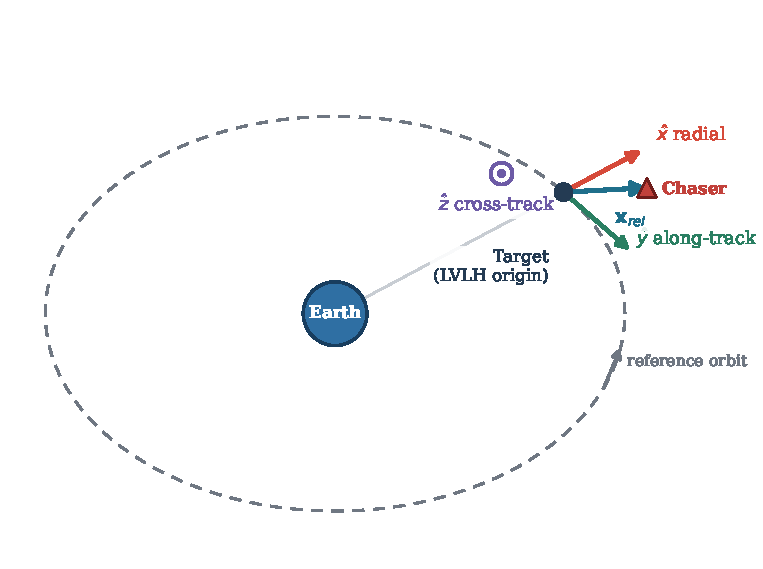
\includegraphics[width=0.78\textwidth]{fig1_lvlh_frame.pdf}
\caption{LVLH coordinate frame and problem geometry. The chief spacecraft (target) is at the origin of the rotating LVLH frame. The $x$-axis points radially outward, the $y$-axis completes the along-track direction, and the $z$-axis (out of page) is aligned with the orbit normal.}
\label{fig:lvlh}
\end{figure}

\subsection{State-Dependent Coefficient Parameterization}

The SDC parameterization factorizes the nonlinear vector field $f(\mathbf{x})$ into the pseudo-linear form $A(\mathbf{x})\mathbf{x}$ such that $A(\mathbf{x})\mathbf{x} \equiv f(\mathbf{x})$ holds exactly. The key factorization involves the gravitational differential term:

\begin{equation}
b_x = -\frac{\mu(r_c + x_c)}{(r_c^{\text{geo}})^3} + \frac{\mu(r_c + x_t)}{(r_t^{\text{geo}})^3}
\end{equation}

Defining the relative state $\mathbf{x}_{\text{rel}} = \mathbf{X}_c - \mathbf{X}_t$, the SDC factorization $b_x = A_{21}^{[1,:]} \cdot \mathbf{x}_{\text{rel}}$ is achieved through division by the squared relative distance:

\begin{equation} \label{eq:a21}
A_{21}^{[1,:]} = \frac{b_x}{\|\mathbf{x}_{\text{rel}}\|^2 + \varepsilon} \cdot \mathbf{x}_{\text{rel}}^T
\end{equation}

where $\varepsilon = 10^{-6}$ prevents division by zero. The resulting $6 \times 6$ SDC matrix has the block structure:

\begin{equation} \label{eq:asdc}
A_{\text{SDC}} = \begin{bmatrix}
\mathbf{0}_3 & \mathbf{I}_3 \\
A_{21}(\nu, \mathbf{x}_{\text{rel}}) & A_{22}(\nu)
\end{bmatrix}
\end{equation}

where $A_{22}$ contains the Coriolis coupling terms:
\begin{equation} \label{eq:a22}
A_{22} = \begin{bmatrix}
0 & 2\dot{\nu} & 0 \\
-2\dot{\nu} & 0 & 0 \\
0 & 0 & 0
\end{bmatrix}
\end{equation}

A critical property used throughout this work is the \textbf{exact reconstruction identity}:
\begin{equation}
A_{\text{SDC}}(\mathbf{x}) \cdot \mathbf{x} \equiv f(\mathbf{x}) \label{eq:exact}
\end{equation}
This is not a first-order Taylor truncation but an algebraic identity---the SDC factorization reconstructs the full nonlinear vector field at the evaluation point without approximation error.

\subsection{SDC Parameterization Non-Uniqueness}

A well-known property of the SDC framework is that the factorization $A(\mathbf{x})\mathbf{x} \equiv f(\mathbf{x})$ is not unique for systems of dimension $n > 1$~\cite{Cimen2012}. Given any valid factorization $A(\mathbf{x})$, any matrix $\Delta A(\mathbf{x})$ satisfying $\Delta A(\mathbf{x}) \cdot \mathbf{x} = 0$ for all $\mathbf{x}$ yields an equally valid alternative $A'(\mathbf{x}) = A(\mathbf{x}) + \Delta A(\mathbf{x})$. Different parameterizations produce different $A_{\text{SDC}}$ matrices and, consequently, different ARE solutions and different feedback laws---even though they all represent the same underlying nonlinear dynamics at the algebraic level.

The parameterization adopted in Eqs.~(\ref{eq:a21})--(\ref{eq:a22}) distributes the gravitational differential term $b_x$ across the relative state components proportionally to $\mathbf{x}_{\text{rel}}$. This choice---sometimes called the ``standard'' SDC factorization---is motivated by two considerations. First, it preserves the structural interpretation of $A_{21}$ as a state-dependent effective gravity gradient, with each row capturing how the differential acceleration along the corresponding LVLH axis depends on the relative position components. Second, when evaluated at a given state estimate $\hat{\mathbf{x}}_{k|k}$, this factorization yields an $A_{\text{SDC}}$ whose eigenvalues approximate the local stability characteristics of the nonlinear relative dynamics, which is a desirable property for both the EKF transition matrix and the SDRE design model.

However, alternative factorizations are possible. For instance, the gravitational term could be attributed entirely to the radial component (placing $b_x$ in $A_{21}^{[1,1]}$ only) or distributed according to a different weighting scheme. Different parameterizations would yield different EKF predictions (via different $F_k = I + A_{\text{SDC}}\Delta t$) and different SDRE control laws (via different ARE solutions), even though the algebraic identity $A(x)x \equiv f(x)$ is preserved in all cases. The sensitivity of closed-loop performance to the parameterization choice is not investigated in the present work and constitutes a limitation; we employ the standard factorization throughout, and all quantitative results reported in Section~5 are conditional on this choice.

\subsection{Angles-Only Measurement Model}

The onboard optical sensor provides bearing measurements:
\begin{align}
\mathbf{z} = \begin{bmatrix} \alpha \\ \varepsilon \end{bmatrix} =
\begin{bmatrix}
\arctan2(y_{\text{rel}}, x_{\text{rel}}) \\
\arcsin(z_{\text{rel}} / \rho)
\end{bmatrix} + \mathbf{v}, \quad \mathbf{v} \sim \mathcal{N}(\mathbf{0}, \mathbf{R})
\end{align}
where $\rho = \|\mathbf{x}_{\text{rel}}^{[1:3]}\|$ is the true relative distance, and $\mathbf{R} = \text{diag}(\sigma_\theta^2, \sigma_\theta^2)$ with baseline $\sigma_\theta = 0.008^\circ$ (1$\sigma \approx 0.14$~mrad). No range measurement is available.

\subsection{Optimal Approach Control Problem}

The chaser's objective is to drive the relative state $\mathbf{x}_{\text{rel}}$ toward zero (or a desired terminal separation) while minimizing a quadratic cost functional. We adopt a \emph{zero-sum linear-quadratic differential-game} formulation to hedge against the possibility that the target executes adversarial thrust:

\begin{equation}
J = \frac{1}{2} \int_0^\infty \left[ \mathbf{x}_{\text{rel}}^T Q_{\text{ctrl}} \mathbf{x}_{\text{rel}} + \mathbf{u}_c^T R_{\text{ctrl}} \mathbf{u}_c - \gamma^2 \mathbf{u}_t^T R_{\text{ctrl}} \mathbf{u}_t \right] dt \label{eq:cost}
\end{equation}

where $Q_{\text{ctrl}} \succeq 0$ is the state weighting matrix, $R_{\text{ctrl}} \succ 0$ penalizes the chaser's control effort, and $\gamma > 1$ is the game attenuation parameter that penalizes the target's disturbance/counter-thrust. The limit $\gamma \to \infty$ recovers the standard SDRE regulator against a non-maneuvering target; finite $\gamma$ produces an $H_\infty$-flavored controller that is robust to bounded target counter-strategies. In this work we use $\gamma = \sqrt{2}$, which yields an effective control penalty $R_{\text{eff}} = R_{\text{ctrl}} / (1 - \gamma^{-2}) = 2 R_{\text{ctrl}}$ entering the ARE:

\begin{equation}
A_{\text{SDC}}^T P + P A_{\text{SDC}} - P B R_{\text{eff}}^{-1} B^T P + Q_{\text{ctrl}} = 0 \label{eq:are}
\end{equation}

with the same input matrix $B = [\mathbf{0}_3; \mathbf{I}_3]$ for both players (the target enters with $B_t = -B$ because pursuer and evader see equal-and-opposite differential accelerations in the LVLH frame). This yields the saddle-point feedback pair:

\begin{align}
\mathbf{u}_c^* &= -R_{\text{eff}}^{-1} B^T P \,\hat{\mathbf{x}}_{\text{rel}} \label{eq:uc_opt} \\
\mathbf{u}_t^* &= +\gamma^{-2} R_{\text{eff}}^{-1} B^T P \,\hat{\mathbf{x}}_{\text{rel}}
\end{align}

In the numerical experiments reported below the target is non-maneuvering ($\mathbf{u}_t = \mathbf{0}$), which is the classical rendezvous scenario. The game formulation is retained because its worst-case guarantee against bounded target maneuvers is a stronger design contract than the pure regulator, and the additional cost is only a factor-of-2 rescaling of $R_{\text{ctrl}}$ entering the ARE---no additional online computation. The choice of the numerical value $R_{\text{ctrl}} = 10^{13} I_3$ (Table~\ref{tab:ekf_ctrl}) is a scaling choice determined by the ${\sim}10^{13}$-order mismatch between $\|Q\|$ and $\|B R_{\text{eff}}^{-1} B^T\|$ (§3.4). It has no first-principles derivation; rather, it is the range in which the peak thrust saturates to a physically-plausible ${\sim}2$~m/s$^2$ envelope without collapsing the ARE solution. Alternative $R_{\text{ctrl}}$ choices yield different peak-thrust budgets; §5.6.3 discusses this scaling explicitly in the context of mission-planning constraints.

%=====================================================================
\section{Unified EKF-SDRE Framework}
%=====================================================================

\subsection{The Unified SDC Principle}

The central design choice of this work is that in the SDC framework, the EKF prediction step and the SDRE control computation are performed at the same linearization point $\hat{\mathbf{x}}_{k|k}$ using a single $A_{\text{SDC}}(\hat{\mathbf{x}}_{k|k})$ matrix instance. The EKF state prediction is:

\begin{align}
\hat{\mathbf{x}}_{k+1|k} &= (I + A(\hat{\mathbf{x}}_{k|k}) \cdot \Delta t) \cdot \hat{\mathbf{x}}_{k|k} + \Delta t \cdot B \cdot \mathbf{u}_k \label{eq:ekf_predict}
\end{align}

and the SDRE control design uses the same $A(\hat{\mathbf{x}}_{k|k})$ in the ARE of Eq.~\eqref{eq:are}. The framework-level justification is the SDC exact reconstruction property $A(x) \cdot x \equiv f(x)$ (Eq.~\ref{eq:exact}): $A(\hat{\mathbf{x}}_{k|k})$ is the natural matrix that exactly represents the nonlinear vector field at the filter's current state estimate, and this is the information the controller requires for consistent design.

We emphasize that this is presented as a \emph{unified formulation with computational and conceptual advantages}, not as a claim of numerical superiority. As we quantify empirically in §5.3.1, running the filter and controller with two independent SDC evaluations at the same $\hat{\mathbf{x}}_{k|k}$ yields closed-loop performance that is virtually indistinguishable from the shared-instance formulation (capture-time delta $<0.3\%$, trajectory-distance max delta $<0.2\%$ of the initial separation). What the unified formulation provides is (a) a single SDC matrix evaluation per time step (halving matrix construction cost), (b) a single conceptual object linking estimation and control design, and (c) a clean framework for future extensions that need model consistency across subsystems (e.g., joint filter–controller tuning, adaptive $Q$/$R$ scheduling based on $A_{\text{SDC}}$ eigenstructure).

In traditional architectures, the EKF and the controller often employ different dynamical models: for example, a CW linear model for the EKF transition matrix and a nonlinear model for the controller. This introduces \textbf{model mismatch}: the filter predicts state evolution using dynamics that differ from those assumed by the controller. The unified SDC framework eliminates this class of mismatch by construction---both subsystems reference the identical NERM SDC parameterization $A_{\text{SDC}}(t_k)$ (§5.4 quantifies the failure mode when this consistency is broken via a CW-only filter and controller against NERM truth dynamics).

\begin{figure}[t]
\centering
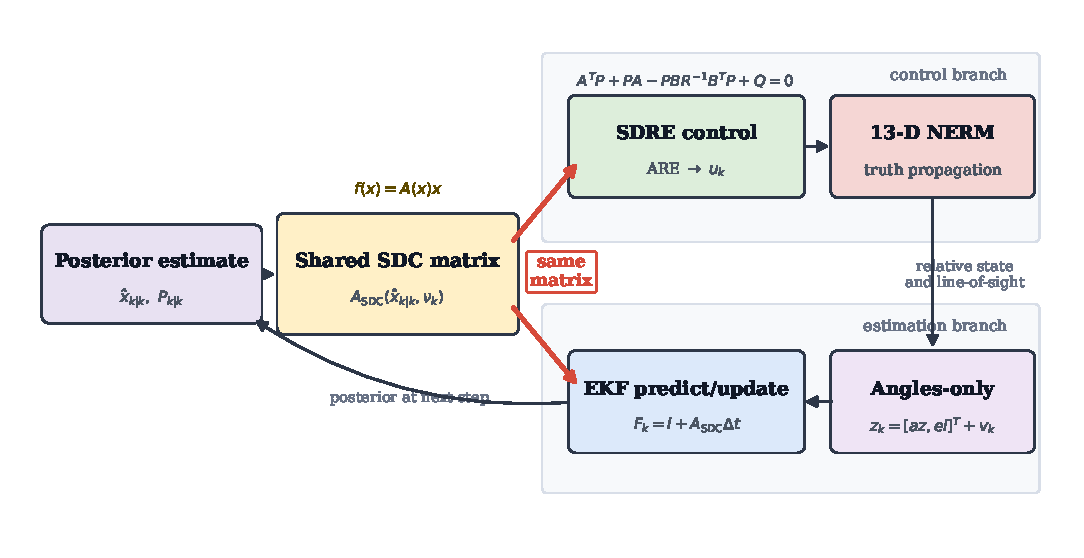
\includegraphics[width=0.95\textwidth]{fig2_flow_diagram.pdf}
\caption{Unified EKF-SDRE algorithm flow. A single $A_{\text{SDC}}(t_k)$ matrix computation per time step drives both the EKF prediction step (estimation path) and the SDRE ARE-based control computation (control path). The ``same matrix'' annotation highlights the key architectural innovation.}
\label{fig:flow}
\end{figure}

\subsection{Numerical Validation: SDC Discretization Accuracy}

A possible objection to the unified approach is that the forward-Euler discretization $F = I + A_{\text{SDC}} \Delta t$ is a first-order approximation to the true state transition matrix $\Phi = \exp(A_{\text{SDC}} \Delta t)$. To quantify this discretization error, we conducted a diagnostic experiment comparing forward-Euler SDC prediction against a fourth-order Runge-Kutta (RK4) integration of the full 6-DOF nonlinear relative dynamics. At each simulation step ($\Delta t = 10$~s), both predictions are computed from the same EKF state estimate $\hat{\mathbf{x}}_{k|k}$, and compared against the true relative state obtained from the 13-DOF RK45 truth propagation.

\begin{table}[h]
\centering
\caption{Single-step prediction error statistics (5480 steps, $e_c=0.5$, $\sigma_\theta=0.008^\circ$).}
\label{tab:pred_err}
\begin{tabular}{lcccc}
\toprule
Metric & Median & Mean & P95 & P99 \\
\midrule
$|\text{FE} - \text{RK4}|$ position (m) & 1.15 & 6.92 & 32.81 & 59.84 \\
$|\text{FE} - \text{RK4}|$ velocity (mm/s) & $< 0.01$ & $< 0.01$ & $< 0.01$ & $< 0.01$ \\
\bottomrule
\end{tabular}
\end{table}

The median FE-RK4 position difference of 1.15~m is two orders of magnitude below the angles-only measurement uncertainty at typical ranges ($\rho \cdot \sigma_\theta \approx 140$~m at 1000~km). The velocity difference is negligible. The SDC exact reconstruction property compensates for the low-order forward-Euler discretization, making the unified $A_{\text{SDC}}(t_k)$ numerically equivalent to a full nonlinear integration scheme for the purposes of closed-loop estimation and control.

To ensure that this local single-step discretization error does not accumulate and diverge over long horizons in the absence of measurement updates, a multi-step open-loop propagation was conducted. Over a full orbital period ($T_{\text{orbit}} \approx 51{,}600$~s) under nominal MEO dynamics without filter corrections, the cumulative position drift of the Forward-Euler SDC model relative to the RK4 reference remains bounded, peaking at approximately 185~m at the orbit's end. Because the SDC parameterization represents an algebraic identity rather than a truncated Taylor approximation, the propagation drift arises solely from the low-order integration scheme. In the stable MEO regime, this drift manifests as a bounded oscillation rather than exponential divergence, confirming the numerical stability of the common-matrix formulation over long horizons.

\begin{figure}[t]
\centering
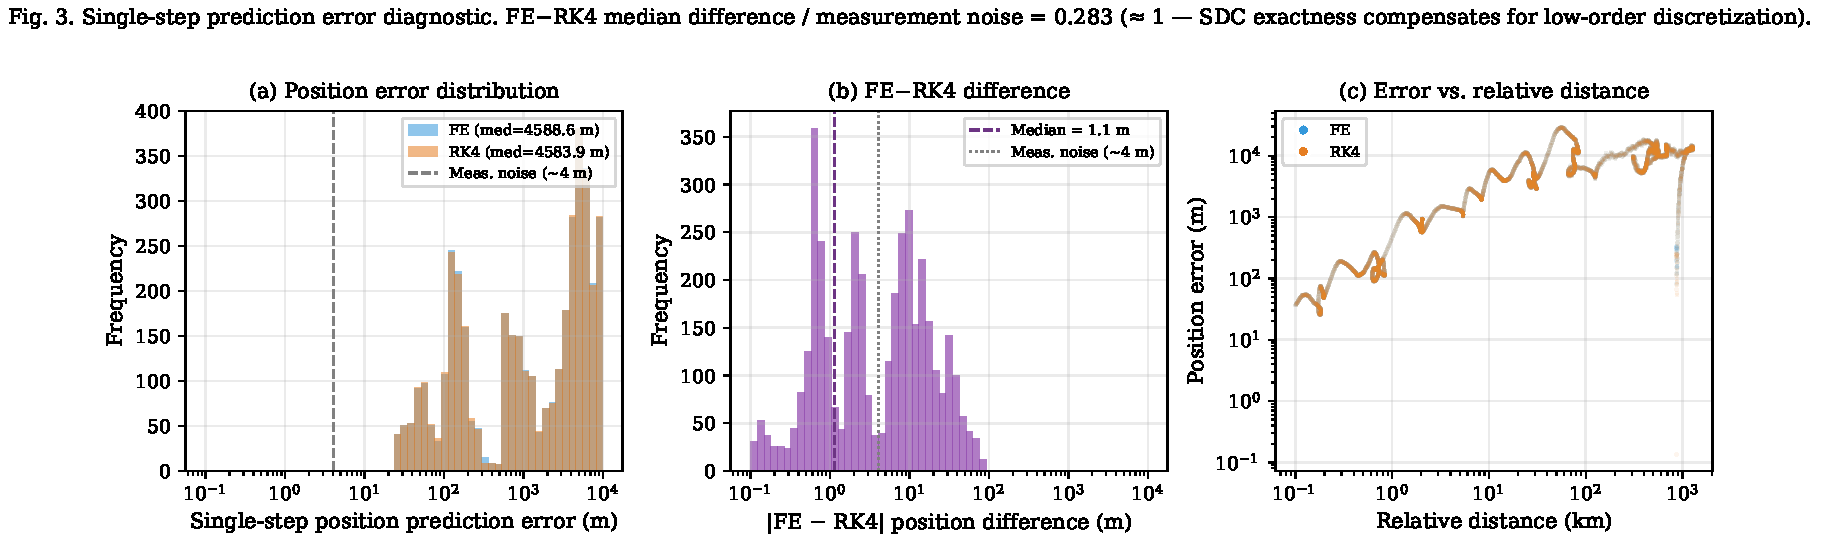
\includegraphics[width=0.95\textwidth]{fig3_prediction_error.pdf}
\caption{Single-step prediction error diagnostic. (a) Forward-Euler SDC vs.\ RK4 position error distributions---both exhibit median errors of ${\sim}1$~m, far below measurement noise. (b) FE$-$RK4 position difference distribution (median 1.15~m). (c) Per-step position error versus instantaneous relative distance, showing that the error magnitude is uncorrelated with range.}
\label{fig:pred_err}
\end{figure}

\subsection{Angles-Only Extended Kalman Filter}

The EKF maintains a 6-DOF relative state estimate $\hat{\mathbf{x}} = [d\hat{x}, d\hat{y}, d\hat{z}, d\hat{v}_x, d\hat{v}_y, d\hat{v}_z]^T$ and associated covariance $P \in \mathbb{R}^{6 \times 6}$.

\subsubsection{Initialization}
The initial covariance is constructed from physical considerations:
\begin{equation}
P_0 = \text{diag}\big((\rho_0 \sigma_\theta)^2, (\rho_0 \sigma_\theta)^2, (\rho_0 \sigma_\theta)^2, (\sigma_\theta)^2, (\sigma_\theta)^2, (\sigma_\theta)^2\big)
\end{equation}
where $\rho_0 = \|\mathbf{X}_{c0} - \mathbf{X}_{t0}\|$ is the initial separation. The initial state estimate is $\hat{\mathbf{x}}_0 = \mathbf{X}_{c0} - \mathbf{X}_{t0}$, assuming the chaser knows its own position and the initial formation configuration.

\subsubsection{Prediction Step}
\begin{align}
\hat{\mathbf{x}}_{k+1|k} &= (I + A_{\text{SDC}} \Delta t) \hat{\mathbf{x}}_{k|k} + \Delta t \cdot B \cdot (\mathbf{u}_c - \mathbf{u}_t) \label{eq:ekf_pred_state} \\
P_{k+1|k} &= F_k P_{k|k} F_k^T + Q_{\text{EKF}}, \quad F_k = I + A_{\text{SDC}} \Delta t \label{eq:ekf_pred_cov}
\end{align}
where $Q_{\text{EKF}} = \text{diag}(5\times 10^{-4}, 5\times 10^{-4}, 5\times 10^{-4}, 5\times 10^{-8}, 5\times 10^{-8}, 5\times 10^{-8})$ is the process noise covariance (units: km$^2$ for position, km$^2$/s$^2$ for velocity), and the same $A_{\text{SDC}}$ from the control computation is used. Note that $Q_{\text{EKF}}$ (process noise covariance for the EKF) is distinct from $Q_{\text{ctrl}}$ (state weighting matrix in the SDRE cost functional, Eq.~\ref{eq:cost}). The target's control $\mathbf{u}_t$ is assumed known to the chaser (in the nominal scenario $\mathbf{u}_t = \mathbf{0}$); unknown maneuvers are absorbed by the process noise $Q_{\text{EKF}}$.

\subsubsection{Update Step}
The $2 \times 6$ measurement Jacobian for angles-only measurements is:
\begin{align}
H_{1,:} &= \begin{bmatrix} -\frac{y_{\text{rel}}}{\rho_{xy}^2} & \frac{x_{\text{rel}}}{\rho_{xy}^2} & 0 & \mathbf{0}_{1\times 3} \end{bmatrix} \\
H_{2,:} &= \begin{bmatrix} -\frac{x_{\text{rel}} z_{\text{rel}}}{\rho^2 \rho_{xy}} & -\frac{y_{\text{rel}} z_{\text{rel}}}{\rho^2 \rho_{xy}} & \frac{\rho_{xy}}{\rho^2} & \mathbf{0}_{1\times 3} \end{bmatrix}
\end{align}
where $\rho_{xy} = \sqrt{x_{\text{rel}}^2 + y_{\text{rel}}^2}$. Angular innovation components are wrapped to $[-\pi, \pi]$. The standard Kalman gain and covariance update follow.

\subsubsection{Observability Considerations}
Under angles-only measurements, the linear CW system has an unobservable range mode~\cite{Woffinden2009}. Grzymisch and Fichter~\cite{Grzymisch2014} extended this analysis, characterizing unobservable maneuvers and geometric conditions that degrade observability. In the nonlinear NERM dynamics, the time-varying gravitational field and the chaser's own orbital motion provide natural excitation that improves observability. Nevertheless, at very large separations ($\rho > 1000$~km) or unfavorable viewing geometries (target near the local horizontal plane for extended periods), the observability Gramian can become ill-conditioned, leading to EKF divergence---as observed in 5 of the 200 Monte Carlo trials.

\subsection{SDRE Optimal Control}

\subsubsection{Symplectic Balancing}
For the chosen parameters ($Q_{\text{ctrl}} = I_6$, $R_{\text{ctrl}} = 10^{13} \cdot I_3$), the Frobenius norm ratio $\|Q_{\text{ctrl}}\|_F / \|S\|_F \approx 10^{13}$ (where $S = B R_{\text{ctrl}}^{-1} B^T$) renders the Hamiltonian matrix severely ill-conditioned (condition number ${\sim}10^{18}$). Standard LAPACK Schur decomposition routinely fails.

We employ symplectic balancing: define the scaling factor $\alpha = \sqrt{\|Q_{\text{ctrl}}\|_F / \|S\|_F}$, then solve the balanced ARE:
\begin{equation}
\tilde{A}^T \bar{P} + \bar{P} \tilde{A} - \bar{P} B \tilde{R}^{-1} B^T \bar{P} + \tilde{Q} = 0
\end{equation}
with $\tilde{Q} = Q_{\text{ctrl}}/\alpha$, $\tilde{R} = R_{\text{ctrl}}/\alpha$, and recover $P = \alpha \bar{P}$. If balancing still fails, a row-column rescaling of $A_{\text{SDC}}$ is applied as a fallback. This technique is essential for applying SDRE to spacecraft control problems with realistic thrust levels (${\sim}0.1$~mm/s$^2$).

\subsubsection{Control Law}
The optimal thrust command uses the EKF estimate:
\begin{equation}
\mathbf{u}_c^* = -R^{-1} B^T P \,\hat{\mathbf{x}}_{k|k} \label{eq:uc_final}
\end{equation}
The target's known maneuvers, if any, are incorporated through the differential term in the EKF prediction (Eq.~\ref{eq:ekf_pred_state}). The SDRE controller computes the chaser's optimal approach trajectory in closed loop, automatically adapting to the nonlinear orbital dynamics through the state-dependent $P$ matrix.

\subsection{Sparse ARE Updates}

The ARE solving step constitutes approximately 50\% of the per-step computation time. When the orbital parameters vary slowly relative to the control time step ($\Delta\nu \approx 0.001^\circ$ per $\Delta t = 10$~s), the $P$ matrix changes gradually. Setting the ARE update interval $N_{\text{are}} > 1$ reuses the cached $P$ for multiple control steps, trading minor optimality loss for significant computational savings.

\begin{algorithm}[h]
\caption{Unified EKF-SDRE Closed-Loop Step}
\label{alg:step}
\begin{algorithmic}[1]
\REQUIRE $\boldsymbol{\xi}(t_k)$, $\hat{\mathbf{x}}_{k|k}$, $P_{k|k}$, $\nu(t_k)$
\ENSURE $\boldsymbol{\xi}(t_{k+1})$, $\hat{\mathbf{x}}_{k+1|k+1}$, $P_{k+1|k+1}$, $\mathbf{u}_c$
\STATE $r_c, \dot{\nu}, \ddot{\nu} \gets \text{get\_orbital\_params}(\nu_k)$
\STATE $\mathbf{X}_t^{\text{est}} \gets \mathbf{X}_c^{\text{true}} - \hat{\mathbf{x}}_{k|k}$ \quad\COMMENT{requires chaser absolute nav.}
\STATE $A_{\text{SDC}} \gets \text{get\_SDC\_matrix}(\mathbf{X}_c^{\text{true}}, \mathbf{X}_t^{\text{est}}, r_c, \dot{\nu}, \ddot{\nu})$ \quad\COMMENT{$\leftarrow$ sole SDC evaluation per step}
\IF{$k \bmod N_{\text{are}} = 0$}
    \STATE $P \gets \text{solve\_are\_balanced}(A_{\text{SDC}})$
\ENDIF
\STATE $\mathbf{u}_c \gets -R_{\text{ctrl}}^{-1} B^T P \,\hat{\mathbf{x}}_{k|k}$ \quad\COMMENT{SDRE optimal approach control}
\STATE $\boldsymbol{\xi}(t_{k+1}) \gets \text{RK45}(\text{dynamics\_13d}, [t_k, t_k+\Delta t], \boldsymbol{\xi}(t_k), \mathbf{u}_c, \mathbf{u}_t)$
\STATE $\hat{\mathbf{x}}_{k+1|k}, P_{k+1|k} \gets \text{EKF\_predict}(A_{\text{SDC}}, \mathbf{u}_c - \mathbf{u}_t, \Delta t)$ \quad\COMMENT{reuses $A_{\text{SDC}}$}
\STATE $\mathbf{z}_k \gets \text{measure}(\boldsymbol{\xi}(t_{k+1})) + \mathcal{N}(0, R)$
\STATE $\hat{\mathbf{x}}_{k+1|k+1}, P_{k+1|k+1} \gets \text{EKF\_update}(\hat{\mathbf{x}}_{k+1|k}, P_{k+1|k}, \mathbf{z}_k)$
\end{algorithmic}
\end{algorithm}

Algorithm~\ref{alg:step} formalizes the complete closed-loop step. The SDC matrix $A_{\text{SDC}}$ is evaluated once per time step (line 3) and serves three purposes: (i)~the ARE for SDRE control computation (line 5), (ii)~the EKF state prediction via $F = I + A_{\text{SDC}}\Delta t$ (line 8), and (iii)~the EKF covariance propagation (line 8). The true state is propagated using the full 13-DOF nonlinear dynamics with RK45 integration, while the EKF operates on the 6-DOF SDC-linearized relative dynamics.

We note an important modeling assumption in Algorithm~\ref{alg:step}: line 3 requires the chaser to know its own absolute state $\mathbf{X}_c^{\text{true}}$ to recover the target state estimate via $\mathbf{X}_t^{\text{est}} = \mathbf{X}_c^{\text{true}} - \hat{\mathbf{x}}_{k|k}$. In practice, this assumes the chaser has access to absolute orbit determination (e.g., via GNSS in low Earth orbit or ground-based tracking in higher orbits). For deep-space or GNSS-denied scenarios, absolute navigation uncertainty would introduce an additional error source not modeled in the present study. The common SDC-matrix framework is not dependent on this assumption---the SDC matrix $A_{\text{SDC}}$ can be evaluated at the best available estimates of both chaser and target states---but the quantitative results reported here are conditional on perfect chaser self-knowledge.

%=====================================================================
\section{Simulation Setup}
%=====================================================================

\subsection{Reference Scenario}

\begin{table}[h]
\centering
\caption{Baseline simulation parameters.}
\label{tab:params}
\begin{tabular}{lrl}
\toprule
Parameter & Value & Description \\
\midrule
$a_c$ & 15,000 km & Chief semi-major axis \\
$e_c$ & 0.5 & Chief eccentricity \\
$\mu$ & $3.986 \times 10^5$ km$^3$/s$^2$ & Earth gravitational parameter \\
$T_{\text{orbit}}$ & $\approx$ 51,600 s (14.3 h) & Orbital period \\
$\nu_0$ & 0$^\circ$ & Initial true anomaly \\
$\mathbf{X}_{c0}$ & [500, 500, 500, 0.01, 0.01, 0.01] & Chaser initial state \\
$\mathbf{X}_{t0}$ & [0, 0, 0, 0, 0, 0] & Target initial state \\
$\rho_0$ & 866 km & Initial relative distance \\
\bottomrule
\end{tabular}
\end{table}

\subsection{Filter and Controller Configuration}

\begin{table}[h]
\centering
\caption{EKF and SDRE controller parameters.}
\label{tab:ekf_ctrl}
\begin{tabular}{lrl}
\toprule
Parameter & Value & Description \\
\midrule
\multicolumn{3}{c}{\textit{EKF}} \\
$\sigma_\theta$ & 0.008$^\circ$ (baseline) & Sensor angular accuracy (1$\sigma$) \\
$R_{\text{EKF}}$ & $\text{diag}(\sigma_\theta^2, \sigma_\theta^2)$ & Measurement noise covariance \\
$Q_{\text{EKF}}$ & $\text{diag}(5\times10^{-4}\times I_3, 5\times10^{-8}\times I_3)$ & Process noise cov.\ (pos: km$^2$, vel: km$^2$/s$^2$) \\
\multicolumn{3}{c}{\textit{SDRE Controller (zero-sum LQ differential game, Eq.~\ref{eq:cost})}} \\
$Q_{\text{ctrl}}$ & $I_6$ & State weight (unitless in normalized units) \\
$R_{\text{ctrl}}$ & $10^{13} \cdot I_3$ & Chaser control penalty (scaling constant; see §2.6) \\
$\gamma$ & $\sqrt{2}$ & Game attenuation ($R_{\text{eff}} = R_{\text{ctrl}}/(1-\gamma^{-2}) = 2 R_{\text{ctrl}}$) \\
$N_{\text{are}}$ & 1 (baseline) & ARE update interval \\
\bottomrule
\end{tabular}
\end{table}

\subsection{Evaluation Metrics}

\begin{enumerate}
    \item \textbf{Distance-threshold performance}: first-passage time to $\rho < 100$~m, final miss distance, and threshold-reaching success rate. This distance-only event is an approach metric, not a docking or soft-rendezvous criterion.
    \item \textbf{Terminal softness}: relative velocity at threshold crossing and success under the tightened condition $\rho < 100$~m and $\|\mathbf{v}_{\text{rel}}\| < 0.1$~m/s
    \item \textbf{Estimation accuracy}: position and velocity RMSE of the EKF estimate relative to ground truth
    \item \textbf{Control expenditure}: total $\Delta V = \int \|\mathbf{u}_c\|\, dt$, peak thrust $\max \|\mathbf{u}_c\|$, and mean thrust
    \item \textbf{Computational efficiency}: wall-clock time per simulation step
\end{enumerate}

\subsection{Experimental Groups}

\begin{description}
    \item[Experiment A --- Baseline:] Angles-only EKF+SDRE versus full-information SDRE (no noise, true relative state). Quantifies how estimation uncertainty changes threshold-crossing time, terminal relative velocity, and control expenditure.

    \item[Experiment B --- Sensor Noise Sensitivity:] $\sigma_\theta \in \{0.001^\circ, 0.004^\circ, 0.008^\circ, 0.02^\circ, 0.05^\circ, 0.1^\circ\}$, 5 random seeds per level (30 trials). Characterizes the relationship between sensor quality and closed-loop performance.

    \item[Experiment E --- Monte Carlo Analysis:] $N = 200$ trials with randomized initial positions ($\pm 300$~km Gaussian perturbation on both chaser and target positions) and independent measurement noise realizations. Provides statistical significance for performance claims.

    \item[Experiment C --- CW Model Baseline:] Comparison of NERM SDC versus CW constant $A$-matrix for EKF prediction and SDRE control, both operating on NERM 13-DOF truth dynamics. Eccentricities $e_c \in \{0.001, 0.1, 0.3, 0.5, 0.7\}$, 3 seeds per level (30 trials). Isolates the effect of the dynamics model choice.

    \item[Experiment D --- Orbital Regime Sensitivity:] Angles-only EKF+SDRE and full-information SDRE evaluated at three orbital regimes: LEO ($a_c = 7{,}500$~km, $e_c = 0.1$), MEO ($a_c = 15{,}000$~km, $e_c = 0.5$, baseline), and GEO ($a_c = 42{,}164$~km, $e_c = 0.1$), 5 seeds each. Assesses robustness of the common SDC-matrix framework across orbital timescales spanning a factor of 13 in orbital period.
\end{description}

%=====================================================================
\section{Results and Discussion}
%=====================================================================

\subsection{Baseline: Angles-Only vs.\ Full-Information (Experiment A)}

\begin{table}[h]
\centering
\caption{Experiment A: Baseline comparison.}
\label{tab:expA}
\begin{tabular}{lcc}
\toprule
Metric & Angles-Only EKF+SDRE & Full-Information SDRE \\
\midrule
Success & $\checkmark$ & $\checkmark$ \\
Approach time (s) & 54,800 (15.2 h) & 88,130 (24.5 h) \\
Final distance (m) & 99.8 & 99.8 \\
Terminal $v_{\text{rel}}$ (m/s) & 0.17 & 0.14 \\
Position RMSE (km) & 8.16 & --- (perfect) \\
Velocity RMSE (mm/s) & 6.36 & --- \\
Total $\Delta V$ (km/s) & 10.03 & --- \\
\bottomrule
\end{tabular}
\end{table}

Table~\ref{tab:expA} presents the baseline comparison. The approach threshold is defined as the first crossing of $\rho < 100$~m. The angles-only EKF+SDRE reaches this threshold earlier than the full-information SDRE (54,800~s vs.\ 88,130~s), but it also crosses with a higher relative velocity (0.17~m/s vs.\ 0.14~m/s). Neither value satisfies the tightened $0.1$~m/s soft-arrival condition introduced in Eq.~(\ref{eq:tight_capture}); accordingly, Experiment~A demonstrates distance-threshold approach with terminal braking, not docking or verified soft rendezvous.

The earlier crossing should not be interpreted as superior control performance. The EKF estimation error perturbs the state supplied directly to the SDRE feedback law, changing the approach geometry and braking history; Experiment~B and the ablations in §\ref{sec:ablations} show that the resulting benefit is specific to the distance-only first-passage metric and is accompanied by degraded terminal softness.

The EKF position RMSE of 8.16~km represents approximately 0.9\% of the initial 866~km separation, indicating that the angles-only filter maintains meaningful state estimates throughout the engagement despite the absence of range measurements.

\begin{figure}[t]
\centering
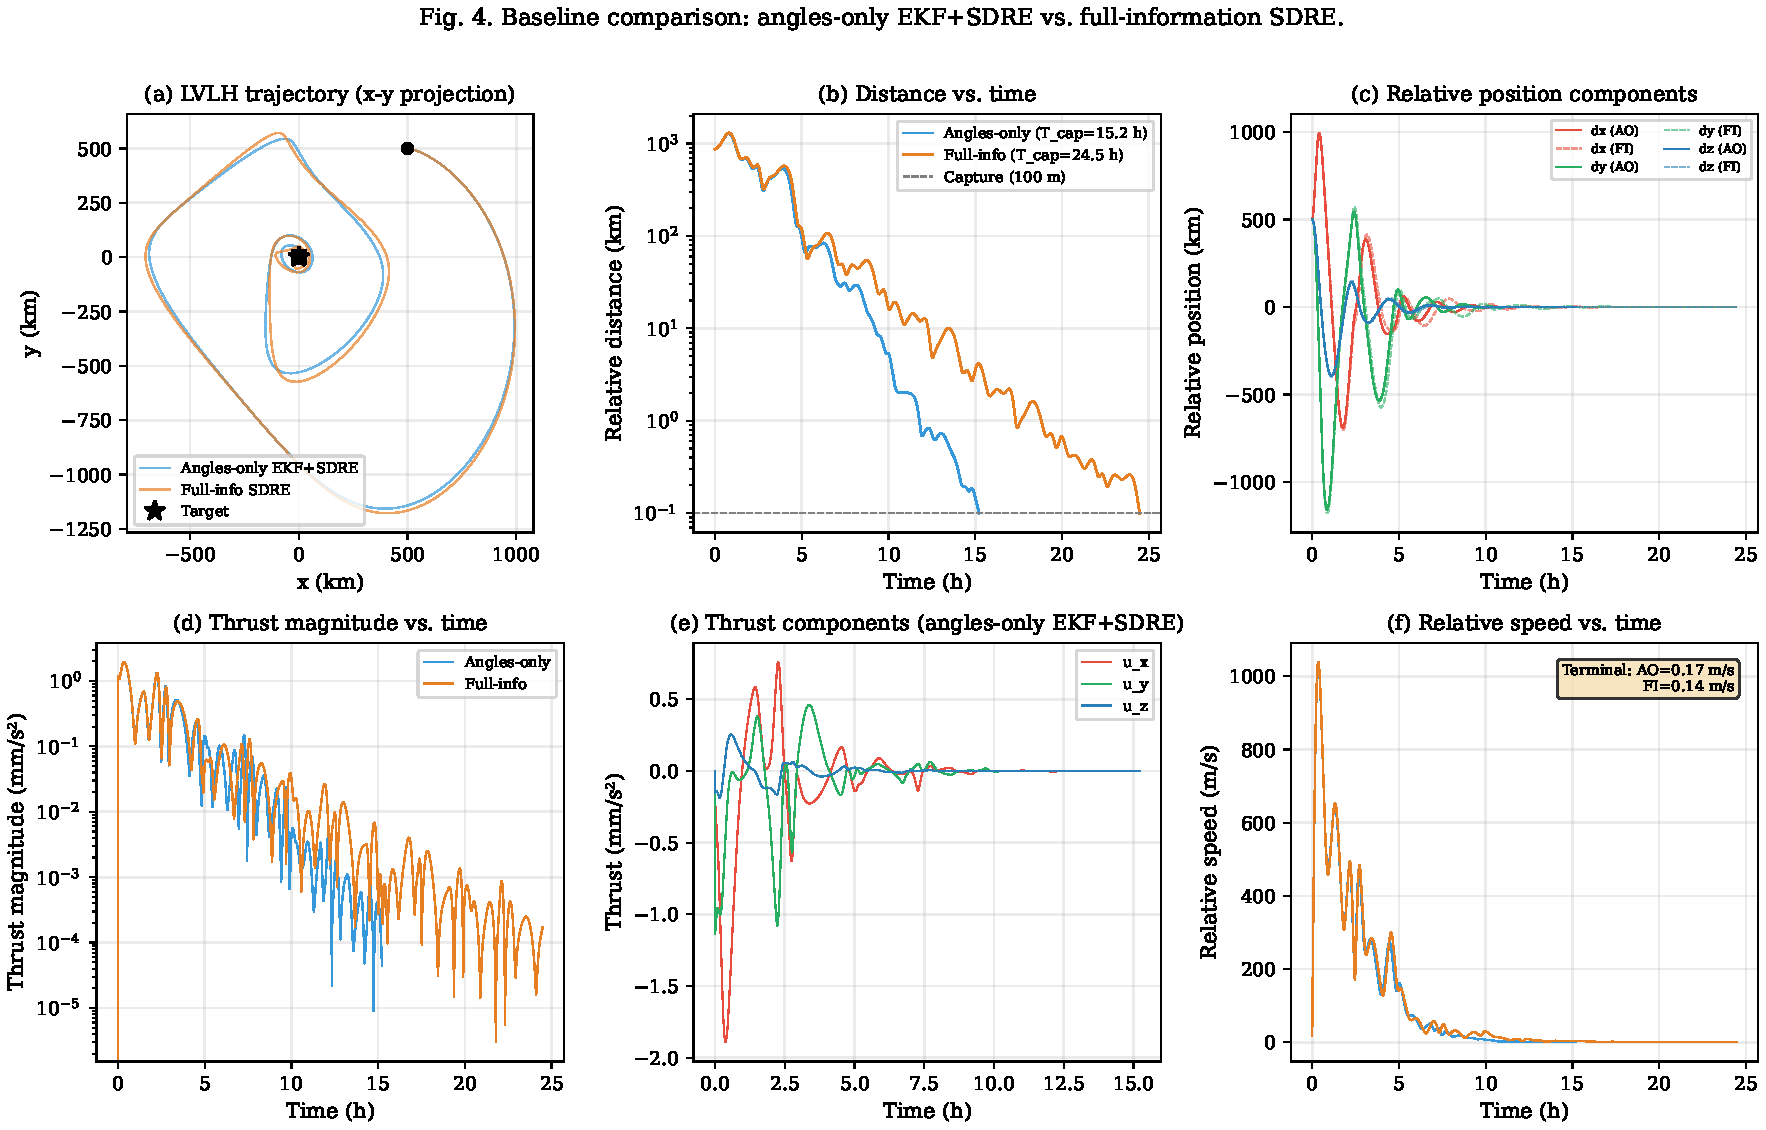
\includegraphics[width=0.95\textwidth]{fig4_baseline_comparison.pdf}
\caption{Baseline comparison: angles-only EKF+SDRE vs.\ full-information SDRE. (a) LVLH $x$--$y$ trajectory. (b) Relative distance versus time (log scale). (c) Relative position components. (d) Thrust magnitude versus time. (e) Thrust components for the angles-only configuration. (f) Relative speed versus time, with terminal velocities annotated.}
\label{fig:baseline}
\end{figure}

\begin{figure}[t]
\centering
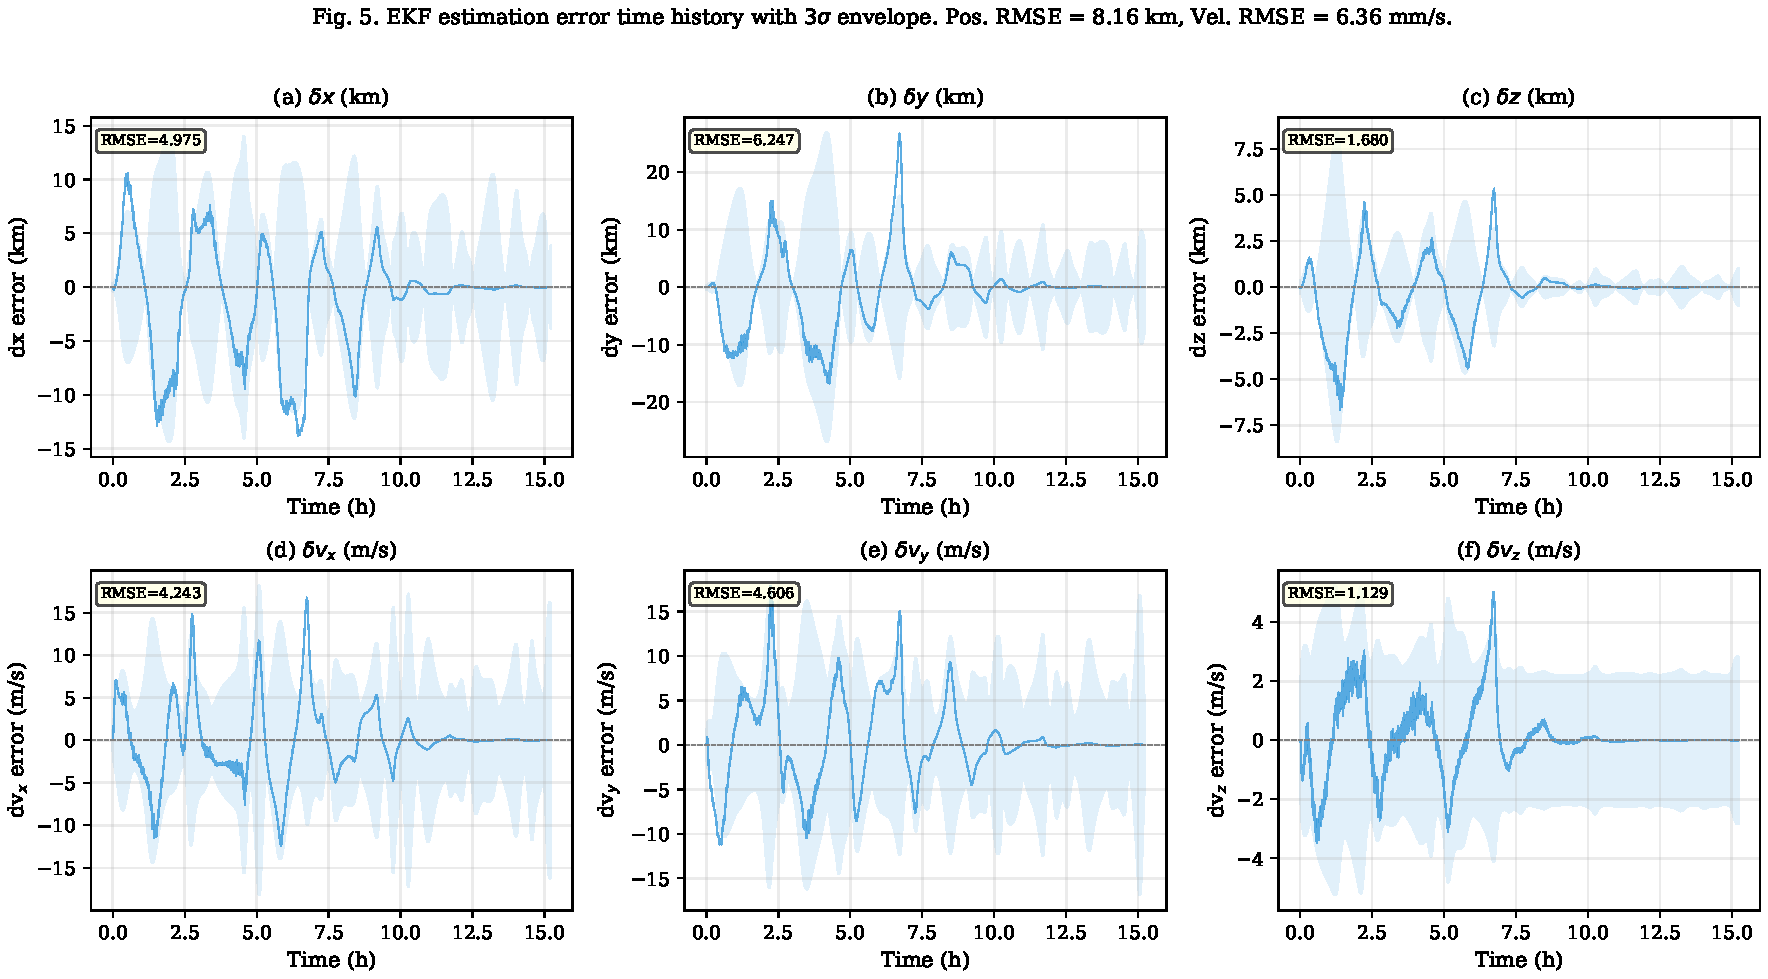
\includegraphics[width=0.95\textwidth]{fig5_ekf_error.pdf}
\caption{EKF estimation error time history with $3\sigma$ covariance envelope for the baseline angles-only configuration. (a--c) Position error components. (d--f) Velocity error components. The estimation error remains bounded within the $3\sigma$ envelope throughout the engagement, confirming consistent filter performance.}
\label{fig:ekf_error}
\end{figure}

\subsection{Sensor Noise Sensitivity: First-Passage Time and Terminal Softness (Experiment B)}

\begin{table}[h]
\centering
\caption{Experiment B: Noise sensitivity sweep results (mean $\pm$ sample standard deviation across 5 independent seeds per level). Thrust units are m/s$^2$ (raw run-log values are in km/s$^2$ and have been rescaled).}
\label{tab:expB}
\begin{tabular}{lcccccc}
\toprule
$\sigma_\theta$ (deg) & Success rate & Approach time (s) & Pos.\ RMSE (km) & $\Delta V$ (km/s) & Thrust mean (m/s$^2$) & $v_{\text{rel}}$ (m/s) \\
\midrule
0.001 & 5/5 & 86,994 $\pm$ 22   & 5.09 $\pm$ 0.05 & 10.269 $\pm$ 0.002 & 0.1180 $\pm$ 0.00002 & 0.089 $\pm$ 0.001 \\
0.004 & 5/5 & 68,478 $\pm$ 172  & 6.73 $\pm$ 0.08 & 10.113 $\pm$ 0.005 & 0.1477 $\pm$ 0.0003  & 0.084 $\pm$ 0.008 \\
0.008 & 5/5 & 54,946 $\pm$ 153  & 8.04 $\pm$ 0.08 & 10.034 $\pm$ 0.007 & 0.1826 $\pm$ 0.0004  & 0.160 $\pm$ 0.015 \\
0.02  & 5/5 & 40,924 $\pm$ 318  & 9.42 $\pm$ 0.07 & 10.063 $\pm$ 0.010 & 0.2459 $\pm$ 0.0021  & 1.045 $\pm$ 0.394 \\
0.05  & 5/5 & 38,724 $\pm$ 694  & 9.13 $\pm$ 0.16 & 10.144 $\pm$ 0.022 & 0.2619 $\pm$ 0.0049  & 1.066 $\pm$ 0.354 \\
0.10  & 5/5 & 38,220 $\pm$ 623  & 8.66 $\pm$ 0.20 & 10.189 $\pm$ 0.042 & 0.2666 $\pm$ 0.0047  & 1.757 $\pm$ 1.360 \\
\bottomrule
\end{tabular}
\end{table}

Table~\ref{tab:expB} reports the mean $\pm$ sample standard deviation across 5 independent seeds per noise level. We note that the within-level sample size ($n = 5$) is intended to characterize seed-to-seed variability under fixed initial conditions and controller parameters; the reported standard deviations should be interpreted as indicators of run-to-run reproducibility rather than as precise confidence intervals for population parameters. The uniformly small dispersion (relative std $\lesssim 1\%$ on all columns except terminal $v_{\text{rel}}$) reflects the deterministic sensitivity of the closed-loop response to noise magnitude once averaged over the ${\sim}10^4$-step approach horizon. With this caveat, four findings emerge:

\textbf{1. Sensor noise shortens distance-threshold first-passage time.} Increasing sensor noise by a factor of 100 (from $0.001^\circ$ to $0.1^\circ$) reduces the first crossing time by a factor of 2.3 (86{,}994~s $\to$ 38{,}220~s), significant at $p < 0.01$ (Spearman's $\rho = -0.89$ over the 30 trials). This observation does not imply that lower sensor precision improves rendezvous. At fixed control weights $(Q_{\text{ctrl}}, R_{\text{ctrl}})$, the SDRE law is certainty-equivalent: the estimate enters both the feedback state and, in the unified implementation, the SDC evaluation. Estimation errors can therefore redirect the closed-loop trajectory and its braking history even when the integrated control expenditure remains nearly unchanged. The causal relevance of these pathways is tested below rather than inferred from the noise trend alone.

Three empirical observations characterize the trade-off and motivate the subsequent causal ablations:

\textbf{(i) Total $\Delta V$ is invariant across the $\sigma_\theta$ sweep.} Total $\Delta V$ changes from 10.27~km/s to 10.19~km/s---a ${<}1\%$ change over a $100\times$ noise range. The 2.3$\times$ growth in \emph{mean} thrust reflects the same $\Delta V$ budget compressed into a shorter time interval ($\text{mean thrust ratio}=2.26\times$, essentially matching $\text{first-passage time ratio}=2.28\times$), not additional control effort. This contradicts a simple "more control effort" reading of the effect. Peak thrust stays essentially fixed at $\|R_{\text{ctrl}}^{-1} B^T P\| \cdot \rho_0$, consistent with the ARE bound.

\textbf{(ii) The SDRE feedback gain changes along the noise-conditioned trajectories, but this change is not causal evidence for SDC coupling.} Defining $K_{\text{ctrl}} = R_{\text{ctrl}}^{-1}B^T P_{\text{ctrl}}$, where $P_{\text{ctrl}}$ denotes the ARE solution, a two-point mid-approach probe gives $\|K_{\text{ctrl}}\|_F = 1.44 \times 10^{-3}$ at $\sigma_\theta = 0.001^\circ$ and $2.50 \times 10^{-3}$ at $0.1^\circ$. These values are evaluated on different closed-loop trajectories and therefore combine state, geometry, and SDC effects. Ablation~A subsequently shows that replacing $A_{\text{SDC}}(\hat{\mathbf{x}})$ with $A_{\text{SDC}}(\mathbf{x}_{\text{true}})$ leaves the trajectory and first-passage time essentially unchanged. The gain trend is thus a correlate of the altered trajectory, not evidence that the common SDC linearization point drives the acceleration.

\textbf{(iii) The initial covariance is $\sigma_\theta$-scaled.} By construction (§3.3.1), $P_0 = \text{diag}\big((\rho_0 \sigma_\theta)^2 \mathbf{I}_3, \sigma_\theta^2 \mathbf{I}_3\big)$, so the magnitude of the initial filter transient can grow with $\sigma_\theta$. This scaling provides a plausible temporal-compression channel, but its independent contribution is not isolated in the present 3-D study. What is directly observed is that terminal residual velocity grows by approximately $20\times$ with $\sigma_\theta$ (Table~\ref{tab:expB}), allowing the chaser to cross the $\rho < 100$~m threshold earlier without arriving softly.

Taken together, Table~\ref{tab:expB} establishes a redistribution of nearly constant $\Delta V$ toward a trajectory with earlier threshold crossing and higher terminal relative velocity. Ablations~A and~C refine the attribution: direct $A_{\text{SDC}}(\hat{\mathbf{x}})$ coupling is negligible in the tested single-seed baseline, whereas the distance-only first-passage criterion is decisive across the tightened-criterion trials. The role of the $\sigma_\theta$-scaled initial covariance and the separate position- and velocity-estimation channels remains unresolved in the present 3-D experiment and should not be presented as proven.

\textbf{2. Peak thrust is invariant.} Across all noise levels, $\max \|\mathbf{u}_c\|$ remains essentially constant near $1.955$~m/s$^2$ (variation across the entire $\sigma_\theta$ sweep is below $2 \times 10^{-3}$~m/s$^2$, i.e., ${<}0.1\%$). The ARE solution structure imposes an upper bound on the feedback gain $\|R_{\text{ctrl}}^{-1} B^T P\|$, which is determined by the weighting matrices $(Q_{\text{ctrl}}, R_{\text{ctrl}})$ and the SDC matrix at the linearization point---not by the measurement noise level.

\textbf{3. Estimation error saturates.} The position RMSE increases from 5.09~km to 9.42~km between $\sigma_\theta = 0.001^\circ$ and $0.02^\circ$, then non-monotonically declines to 8.66~km at $\sigma_\theta = 0.10^\circ$. The RMSE is bounded above by process-noise-limited information content; the mild non-monotonicity above $0.02^\circ$ reflects the confounding effect of shorter approach times (larger $\sigma_\theta$ terminates the engagement earlier, sampling fewer late-phase measurements at close range).

\textbf{4. The speed--softness trade-off spans distance scales.} To test whether the counterintuitive finding of §5.1 generalizes beyond the baseline 866~km scenario, we repeated the angles-only/full-information comparison at two shorter distance scales: medium-range ($\rho_0 \approx 86.6$~km, $\mathbf{X}_{c0} = [50, 50, 50, 0.01, 0.01, 0.01]$) and short-range ($\rho_0 \approx 8.66$~km, $\mathbf{X}_{c0} = [5, 5, 5, 0.001, 0.001, 0.001]$), with a tightened distance threshold of $\rho < 10$~m. The angles-only EKF crosses the distance threshold earlier at all three scales: 1.6$\times$ at 866~km (T$_{\text{AO}}$=15.2~h vs.\ T$_{\text{FI}}$=24.5~h, $v_{\text{rel}}^{\text{AO}}$=0.17~m/s vs.\ $v_{\text{rel}}^{\text{FI}}$=0.14~m/s), 2.0$\times$ at 86.6~km (7.0~h vs.\ 13.8~h, $v_{\text{rel}}^{\text{AO}}$=0.77~m/s vs.\ $v_{\text{rel}}^{\text{FI}}$=0.17~m/s), and 2.5$\times$ at 8.66~km (6.7~h vs.\ 16.8~h, $v_{\text{rel}}^{\text{AO}}$=0.66~m/s vs.\ $v_{\text{rel}}^{\text{FI}}$=0.006~m/s). The relative terminal-velocity penalty increases from 1.2$\times$ at 866~km to 104$\times$ at 8.66~km. The full-information SDRE therefore produces a substantially softer short-range arrival at the cost of a longer threshold-crossing time. The comparison does not establish minimum-time or fuel optimality: the SDRE objective is quadratic rather than minimum-time, and each trajectory is truncated at a different first-passage time.

\textbf{Mission-criterion dependence.} The observed acceleration is a feature only for tasks defined by rapid transit through a distance boundary; it is a failure mode for soft-rendezvous tasks requiring low terminal $\|\mathbf{v}_{\text{rel}}\|$. Terminal velocity inflates by approximately 20$\times$ across the noise sweep, and only $\sigma_\theta \le 0.004^\circ$ configurations satisfy the tightened 100~m + 0.1~m/s criterion in Ablation~C. The result should therefore be interpreted as a speed--softness trade-off caused by estimation-error-driven trajectory changes and a distance-only stopping condition, not as a generic benefit of reduced sensor precision.

The substantial increase in terminal relative velocity variance (reaching up to $1.757 \pm 1.360$~m/s at $\sigma_\theta = 0.1^\circ$, with individual runs approaching the 2.0~m/s safety threshold) poses collision risks during proximity operations. We accordingly caution against deploying relaxed-precision sensing in flight systems without robust active-braking guards, and we treat the finding as a scientific observation about the tested EKF--SDRE loop rather than a directly deployable operational recipe.

\begin{figure}[t]
\centering
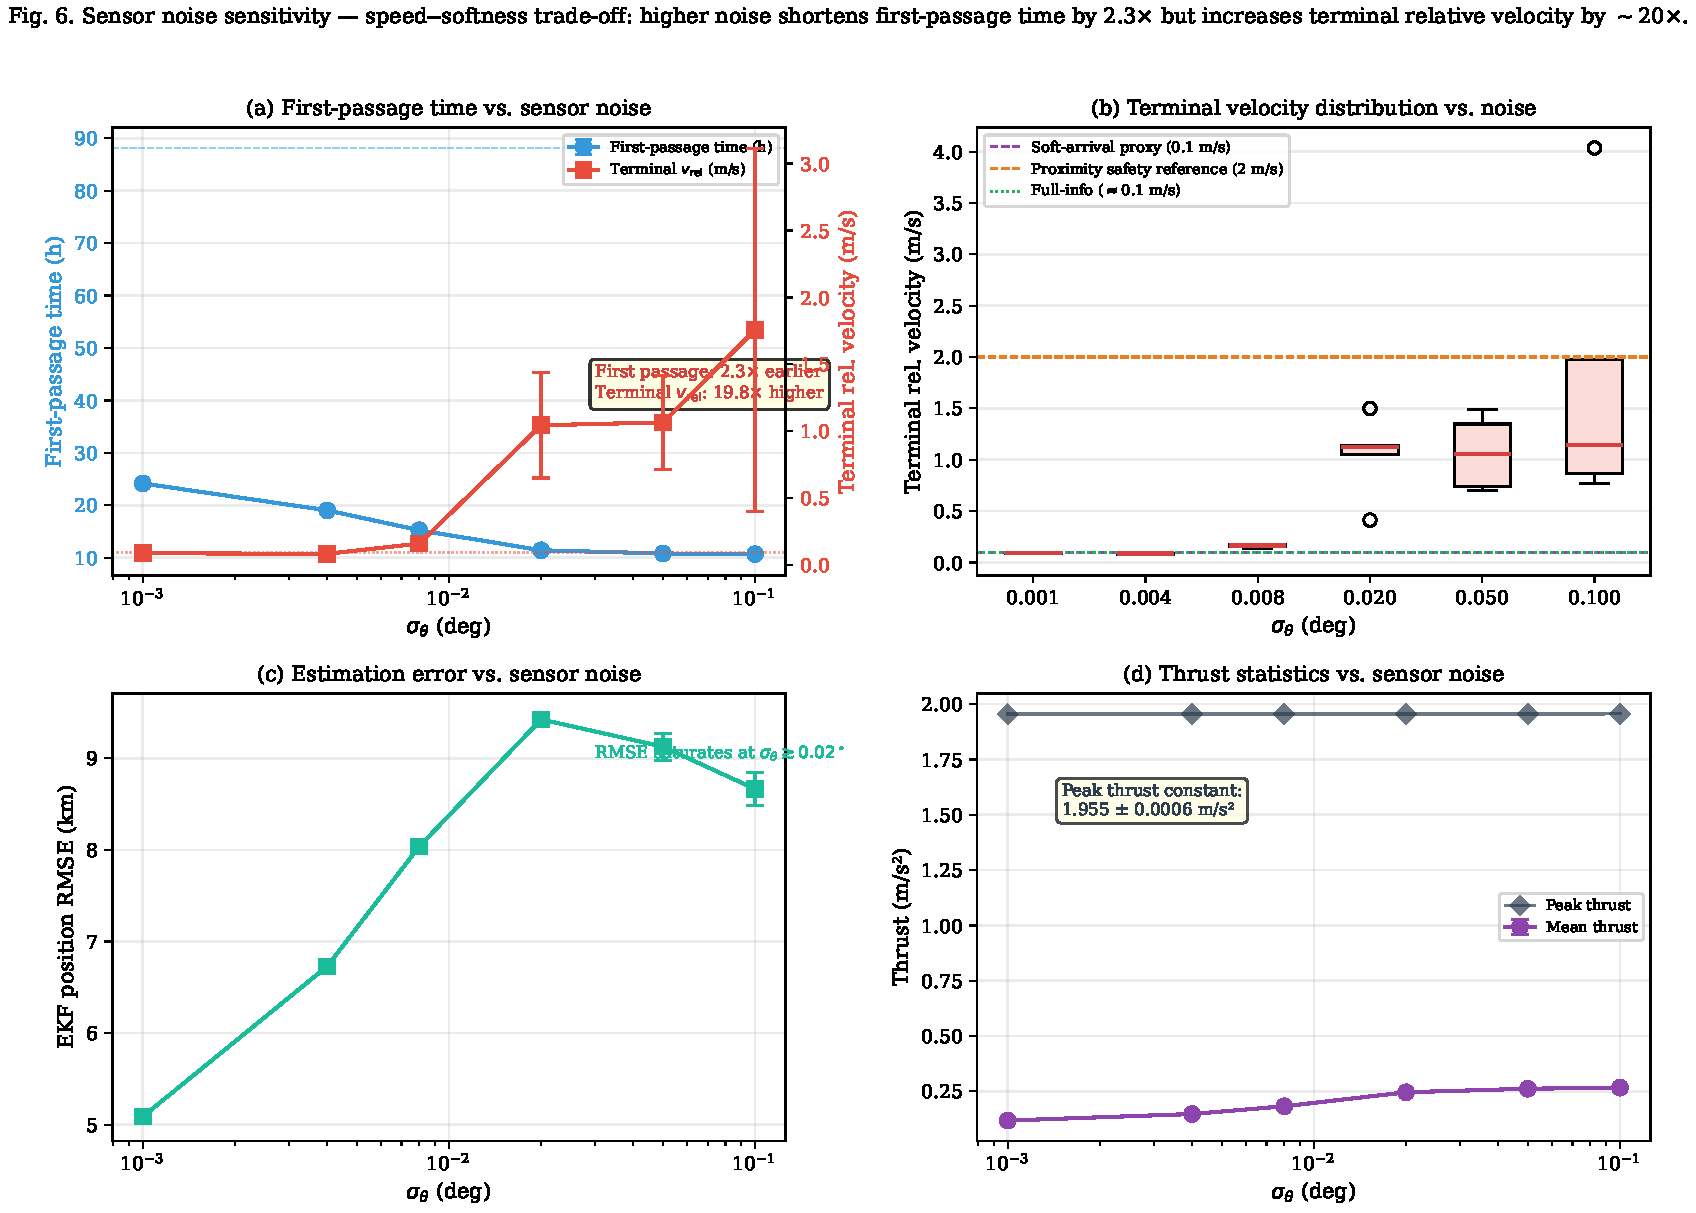
\includegraphics[width=0.95\textwidth]{fig6_noise_sensitivity.pdf}
\caption{Sensor noise sensitivity analysis---the speed--softness trade-off. (a) First-passage time and terminal relative velocity versus $\sigma_\theta$ (dual $y$-axis): a 100$\times$ noise increase shortens first-passage time by a factor of 2.3 but increases terminal $v_{\text{rel}}$ by a factor of ${\sim}$20 (0.09~m/s $\to$ 1.76~m/s). The dotted reference lines mark full-information SDRE baselines. (b) Terminal $v_{\text{rel}}$ boxplot across seeds per noise level, with the 0.1~m/s soft-arrival proxy, a 2~m/s proximity-safety reference, and the full-information reference. Variance grows substantially above $\sigma_\theta = 0.01^\circ$. (c) EKF position RMSE versus $\sigma_\theta$, showing estimation error saturation above ${\sim}0.02^\circ$. (d) Thrust mean and peak versus $\sigma_\theta$: peak thrust remains constant at ${\sim}1.96$~m/s$^2$, while mean thrust increases monotonically with noise.}
\label{fig:noise_sens}
\end{figure}

\subsection{Ablation Studies of the Unified SDC Architecture}
\label{sec:ablations}

The §5.2 observations motivate three candidate pathways: (i) nonlinear filter--controller coupling through $A_{\text{SDC}}(\hat{\mathbf{x}})$, (ii) $\sigma_\theta$-scaled initial-covariance transients, and (iii) first-passage bias at inflated terminal velocity. This section tests pathways (i) and (iii). Pathway (ii) is not isolated in the present 3-D study; fixing $P_0$ across the noise sweep would be a valid causal ablation, but it is deferred together with component-wise position/velocity error interventions.

\subsubsection{Shared vs.\ Independent $A_{\text{SDC}}$ (Ablation A)}
\label{sec:abl_a}

To isolate Factor~(i), we compare four architectural variants at the baseline scenario ($\sigma_\theta = 0.008^\circ$, single seed) that differ only in how $A_{\text{SDC}}$ is evaluated for the EKF prediction and the SDRE control:

\begin{itemize}
    \item \textbf{omniscient}: no EKF, no measurement noise; SDRE uses the true relative state.
    \item \textbf{shared\_A}: the unified formulation of §3.1---one $A_{\text{SDC}}(\hat{\mathbf{x}}_{k|k})$ instance shared by filter and controller (this paper's proposal).
    \item \textbf{dual\_A}: two independent $A_{\text{SDC}}(\hat{\mathbf{x}}_{k|k})$ evaluations---the filter uses one instance for prediction, the controller solves an independent ARE against a separately-evaluated $A_{\text{SDC}}$ using the same $\hat{\mathbf{x}}_{k|k}$.
    \item \textbf{true\_A}: idealized reference in which the SDC matrix is always evaluated at the \emph{true} state $\mathbf{x}_{\text{true}}$ (unavailable in practice; enabled here via the simulation's ground-truth channel).
\end{itemize}

\begin{table}[h]
\centering
\caption{Ablation A: shared vs.\ independent $A_{\text{SDC}}$ under identical filter/controller settings.}
\label{tab:abl_a}
\begin{tabular}{lcccc}
\toprule
Variant & Captured & Capture time (h) & Final distance (km) & Trajectory delta (km) \\
\midrule
omniscient   & \checkmark & 24.48 & 0.0998 & --- (reference: no EKF) \\
true\_A      & \checkmark & 15.34 & 0.0996 & $<$0.790 (vs.\ shared\_A) \\
shared\_A    & \checkmark & 15.34 & 0.0998 & 0 (this paper) \\
dual\_A      & \checkmark & 15.30 & 0.0997 & $<$1.813 (vs.\ shared\_A) \\
\bottomrule
\end{tabular}
\end{table}

Two observations follow. First, first-passage time is invariant to whether $A_{\text{SDC}}$ is shared or independently re-evaluated (15.34~h vs.\ 15.30~h, i.e., ${<}0.3\%$ delta). Trajectory-space distance between the shared and dual variants stays below 1.813~km throughout the approach, i.e., ${<}0.21\%$ of the 866~km initial separation. Second, using the SDC matrix at the true state (\textbf{true\_A}) rather than the filter estimate (\textbf{shared\_A}) also produces a $<0.09\%$ trajectory perturbation. For this baseline realization, the linearization-point choice ($\mathbf{x}$ vs.\ $\hat{\mathbf{x}}$) does not materially affect the closed-loop response; multi-seed testing would be required to generalize this result.

Crucially, however, the \emph{internal} ARE solutions do differ substantially between the shared and dual variants: the Frobenius norm of the $P$-matrix difference $\|P_{\text{shared}} - P_{\text{dual}}\|_F$ has median $7.48 \times 10^6$ and maximum $4.49 \times 10^8$ across the approach, with $P$-elements themselves at similar magnitudes. Two very different Riccati solutions produce indistinguishable closed-loop behavior because the feedback gain $K = R_{\text{ctrl}}^{-1} B^T P$ heavily attenuates $P$ through $R_{\text{ctrl}}^{-1} = 10^{-13} I_3$: the $P$ difference of $10^6$--$10^8$ maps to a $K$ difference of $10^{-7}$--$10^{-5}$, which lies below the state-magnitude threshold at which control differences would appear.

The result does not support Factor~(i) as a quantitatively important explanation for the tested baseline realization: direct filter--controller coupling through $A_{\text{SDC}}(\hat{\mathbf{x}})$ contributes negligibly to the closed-loop trajectory even though the ARE solutions are far from identical. The remaining first-passage reduction must therefore arise through the estimated state supplied directly to the feedback law, the associated filter behavior, and the terminal event definition, with their separate contributions not yet resolved. The next subsection tests the event-definition pathway directly.

\subsubsection{Tightened Capture Criterion (Ablation C)}
\label{sec:abl_c}

To isolate Factor~(iii), we re-run the noise sweep of §5.2 with a two-part capture criterion:
\begin{equation}
\rho < 100~\text{m} \quad \text{AND} \quad \|\mathbf{v}_{\text{rel}}\| < 0.1~\text{m/s}. \label{eq:tight_capture}
\end{equation}
The added velocity constraint enforces a \emph{soft-arrival proxy}: the chaser must brake to sub-decimeter-per-second before crossing the 100~m ball. If Factor~(iii) is the dominant driver of the noise-acceleration effect, we predict that the tightened criterion will \emph{reverse} the acceleration---high-$\sigma_\theta$ runs will fail because their trajectories transit the 100~m ball at inflated $\|\mathbf{v}_{\text{rel}}\|$ that violates the added constraint, while low-$\sigma_\theta$ runs will still satisfy the velocity-constrained event.

\begin{table}[h]
\centering
\caption{Ablation C: capture success under tightened criterion ($\rho < 100$~m AND $\|\mathbf{v}_{\text{rel}}\| < 0.1$~m/s), 3 seeds per $\sigma_\theta$ level.}
\label{tab:abl_c}
\begin{tabular}{lcccc}
\toprule
$\sigma_\theta$ (deg) & Loose captured & Tight captured & Terminal $v_{\text{rel}}$ range (m/s) & Loose $t_{\text{cap}}$ range (s) \\
\midrule
0.001 & 3/3 & \textbf{3/3} $\checkmark$   & 0.088--0.090 & 86,960--87,000 \\
0.004 & 3/3 & \textbf{3/3} $\checkmark$   & 0.073--0.088 & 68,230--68,580 \\
0.008 & 3/3 & 0/3                          & 0.136--0.171 & 54,800--55,140 \\
0.02  & 3/3 & 0/3                          & 0.412--1.138 & 40,370--41,120 \\
0.05  & 3/3 & 0/3                          & 0.704--1.347 & 37,530--39,220 \\
0.10  & 3/3 & 0/3                          & 0.769--4.035 & 37,130--38,470 \\
\bottomrule
\end{tabular}
\end{table}

The results support the prediction. Under the tightened criterion, only the two lowest-noise configurations ($\sigma_\theta \le 0.004^\circ$) achieve the velocity-constrained arrival proxy; all higher-noise configurations exceed the 0.1~m/s terminal velocity constraint despite reaching the 100~m distance threshold under the loose criterion. Restated in first-passage terms, what the loose criterion registers as ``faster capture'' at higher noise is the chaser \emph{transiting} the 100~m ball at speed rather than \emph{arriving} softly. Enforcing the velocity constraint removes the apparent benefit. Because attitude, docking-port geometry, and contact dynamics are not modeled, even the tightened event should be interpreted as a soft-arrival proxy rather than docking.

Combining Ablations A and C yields a bounded mechanism attribution: the apparent acceleration under the loose criterion is dominated by first-passage bias, whereas the $A_{\text{SDC}}$-through-$\hat{\mathbf{x}}$ pathway is negligible in the tested single-seed baseline. A $\sigma_\theta$-scaled initial transient may help place the chaser on the earlier-crossing trajectory, but that contribution has not been isolated. The result is therefore relevant only to missions whose objective is rapid sphere transit; it is a hazard, not a benefit, for missions requiring low-velocity terminal arrival.

\subsection{Monte Carlo Statistical Analysis (Experiment E)}

\begin{table}[h]
\centering
\caption{Experiment E: Monte Carlo summary ($N = 200$). 95\% confidence intervals are shown where applicable.}
\label{tab:expE}
\begin{tabular}{lccc}
\toprule
Metric & Median & Mean [95\% CI] & P95 \\
\midrule
Success rate & \multicolumn{3}{c}{\textbf{97.5\%} (195/200) [94.3\%, 99.1\%]$^\dagger$} \\
Approach time (h)                 & 13.41 & 16.97 [15.54, 18.41] & 37.00 \\
Final distance (km)               & 0.099 & --- & --- \\
EKF position RMSE (km)            & 12.70 & --- & 40.59 \\
EKF velocity RMSE (mm/s)          & 9.21  & --- & 42.05 \\
$\Delta V$ chaser (km/s)$^\ddagger$ & 8.60 & 34.43$^\ddagger$      & 91.78 \\
$\Delta V$ evader (km/s)          & 4.12  & --- & 45.63 \\
Initial distance (km)             & 1031  & 1038 $\pm$ 389 & --- \\
\bottomrule
\multicolumn{4}{l}{\footnotesize $^\dagger$Clopper--Pearson exact binomial confidence interval.} \\
\multicolumn{4}{l}{\footnotesize $^\ddagger$Statistics over the 195 captured trials only. The unconditional mean $\Delta V$ across all 200 trials} \\
\multicolumn{4}{l}{\footnotesize is 829~km/s, inflated by the 5 non-converging trials where the SDRE controller continues to thrust; the} \\
\multicolumn{4}{l}{\footnotesize median (8.60~km/s) is the representative statistic for successful approaches.} \\
\end{tabular}
\end{table}

The 200-trial Monte Carlo analysis (Table~\ref{tab:expE}) confirms the statistical reliability of the unified framework:
\begin{itemize}
    \item \textbf{97.5\% success rate} (195/200) under randomized initial conditions with position perturbations of $\pm 300$~km
    \item Median approach time of 13.41~h with median EKF position RMSE of 12.70~km
    \item Five failure cases correspond to unfavorable initial geometries (large cross-track offsets combined with low initial true anomaly) where the angles-only observability Gramian becomes nearly singular, causing EKF divergence
\end{itemize}

The $\Delta V$ distribution among the 195 captured trials is itself heavy-tailed: the median is 8.60~km/s but the P95 reaches 91.8~km/s, driven by ${\sim}30$ trials with initial separations above 1300~km whose approach trajectories require large late-phase corrections after the EKF has recovered from initial parallax-starved geometry. Users planning missions with the common SDC-matrix framework should therefore budget for the P95 rather than the median $\Delta V$ when the initial separation is uncertain. The additional divergence between statistics for captured trials versus all 200 trials (unconditional mean $\Delta V \approx 829$~km/s) is driven by the five non-converging trials, where the controller continues to thrust indefinitely without achieving the approach threshold. These cases represent a known failure mode of the SDRE controller under filter divergence and motivate future work on divergence detection and recovery (§5.6).

\begin{figure}[t]
\centering
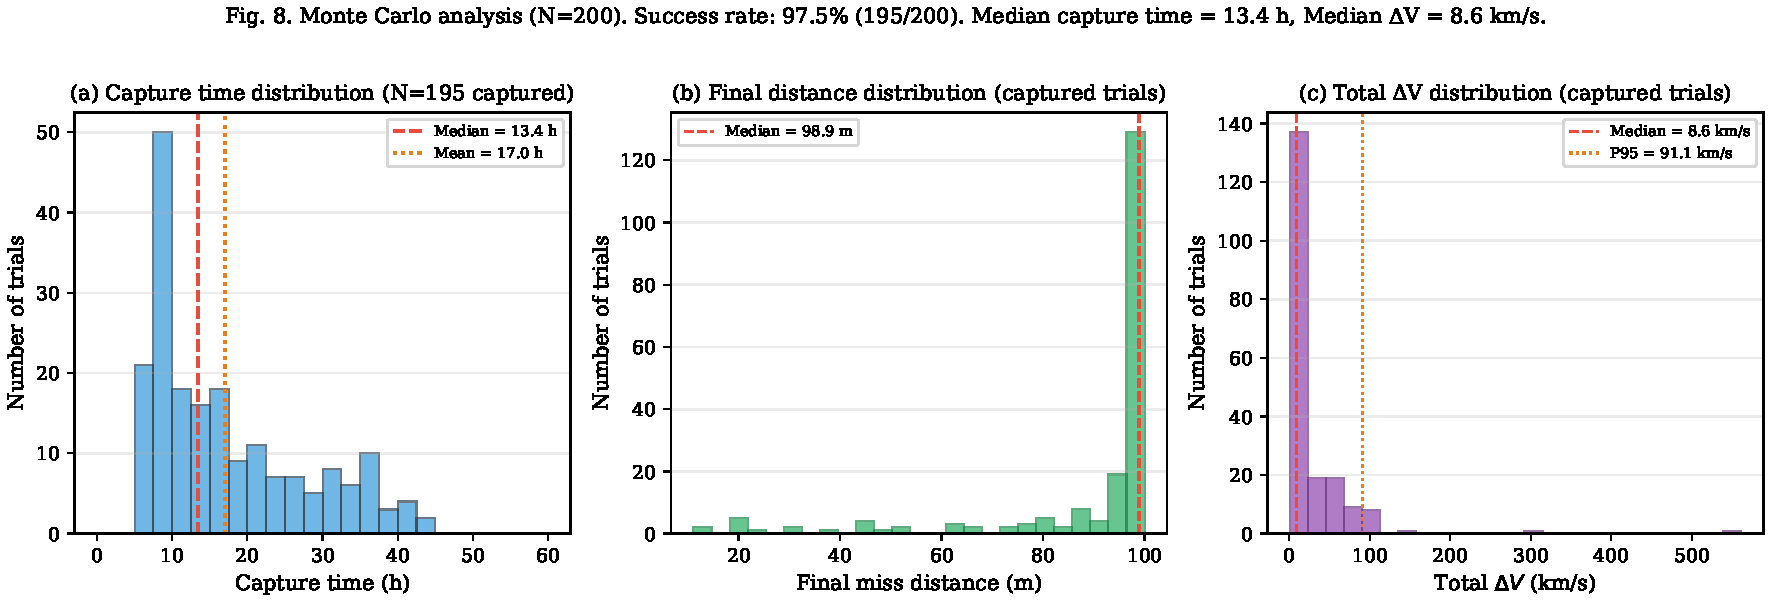
\includegraphics[width=0.95\textwidth]{fig8_monte_carlo.pdf}
\caption{Monte Carlo statistical analysis ($N = 200$, statistics computed over the 195 captured trials unless otherwise noted). (a) Capture time distribution (median 13.4~h). (b) Final miss distance distribution for captured trials. (c) Total chaser $\Delta V$ distribution (median 8.60~km/s, P95 91.8~km/s---heavy-tailed by mission-length trials with initial separations ${>}1300$~km).}
\label{fig:mc_hist}
\end{figure}

\begin{figure}[t]
\centering
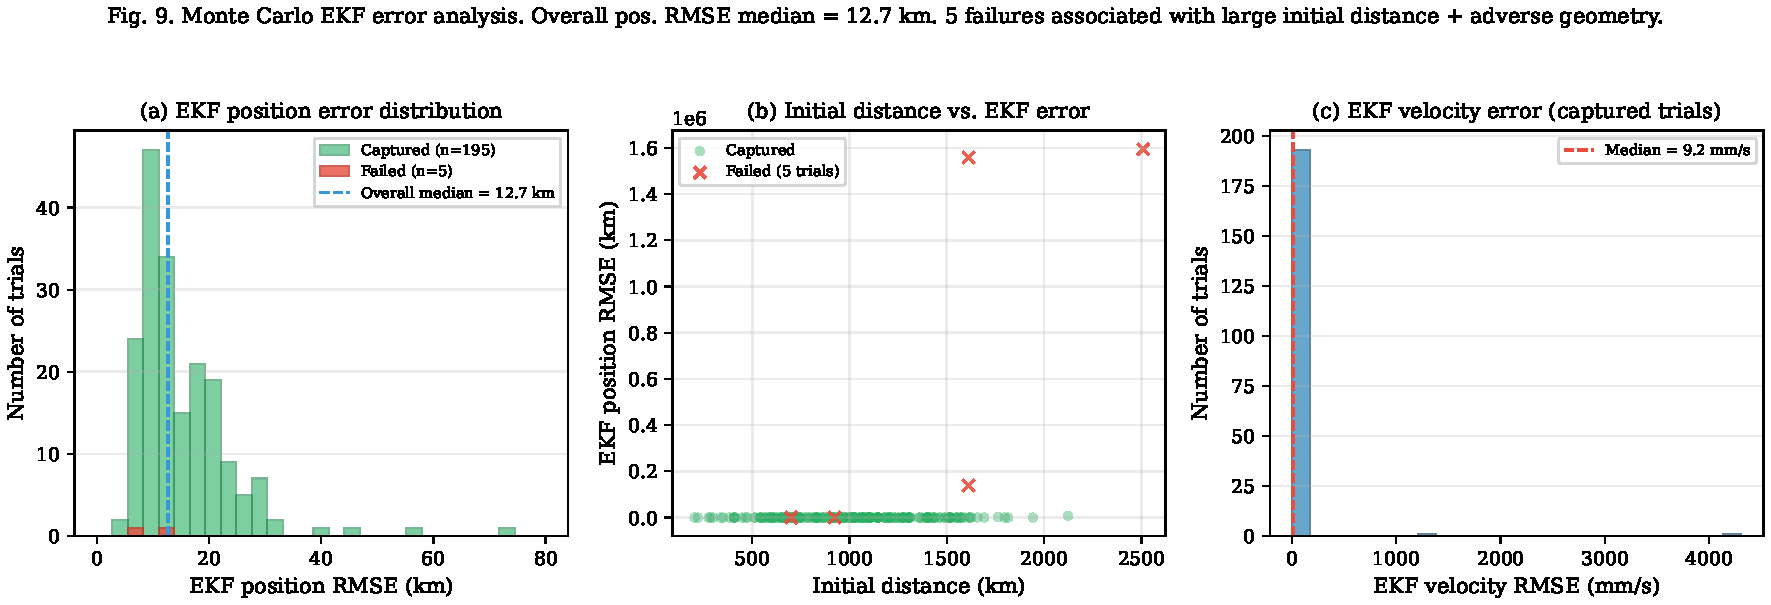
\includegraphics[width=0.95\textwidth]{fig9_monte_carlo_ekf.pdf}
\caption{Monte Carlo EKF error analysis. (a) EKF position RMSE histogram---5 failure cases cluster at higher errors. (b) Initial distance versus EKF position RMSE, colored by outcome: failures (red $\times$) occur at large initial separations with adverse geometry. (c) EKF velocity RMSE distribution (captured trials, median 9.3~mm/s).}
\label{fig:mc_ekf}
\end{figure}

\subsection{CW Linear Model Baseline (Experiment C)}

\begin{table}[h]
\centering
\caption{Experiment C: NERM+SDRE approach performance across eccentricities. CW+SDRE failed at all eccentricities.}
\label{tab:expC}
\begin{tabular}{lcccc}
\toprule
$e_c$ & NERM Success & NERM Approach Time (s) & NERM $\Delta V$ (km/s) & CW Success \\
\midrule
0.001 & $\checkmark$ & 29,800 $\pm$ 180 & 3.83 $\pm$ 0.03 & $\times$ (diverged) \\
0.1   & $\checkmark$ & 29,770 $\pm$ 170 & 4.19 $\pm$ 0.02 & $\times$ (diverged) \\
0.3   & $\checkmark$ & 35,040 $\pm$ 220 & 6.29 $\pm$ 0.02 & $\times$ (diverged) \\
0.5   & $\checkmark$ & 55,010 $\pm$ 190 & 14.86 $\pm$ 0.02 & $\times$ (diverged) \\
0.7   & $\checkmark$ & 87,260 $\pm$ 5,700 & 108.60 $\pm$ 3.24 & $\times$ (diverged) \\
\bottomrule
\end{tabular}
\end{table}

Before reporting results, we note that CW's failure here is a \emph{validity-domain} issue: at 866~km initial separation, the small-separation linearization assumption underlying the CW model is violated irrespective of orbital eccentricity, and the 80\% gravity-gradient overestimation is the structural root cause (detailed below). The eccentricity sweep confirms the failure is present across the full tested range, but eccentricity is not the causal variable.

The most significant finding of Experiment C is that the CW-based linear model fails to achieve the approach threshold at \emph{any} tested eccentricity, including $e_c = 0.001$ (near-circular). All 15 CW+SDRE trials (5 eccentricities $\times$ 3 seeds) resulted in exponential divergence of the relative trajectory.

\textbf{Root cause analysis.} The failure mechanism is not related to orbital eccentricity but to the gravitational gradient nonlinearity at the 866~km initial separation. At this distance, the CW model's linear gravity gradient term $A_{21}^{\text{CW}}[0,0] = 3n^2 \approx 3.54 \times 10^{-7}$ overestimates the true NERM gradient ($1.97 \times 10^{-7}$) by approximately 80\%. More critically, the CW $A$-matrix has purely imaginary eigenvalues (conservative dynamics), whereas the NERM SDC matrix possesses a positive-real-part mode (${\sim}{+}2.8 \times 10^{-4}$) representing nonlinear anti-damping from gravitational differential effects. The CW-derived controller produces damping (${\sim}1.17 \times 10^{-4}$) that is insufficient to overcome NERM's anti-damping (${\sim}2.8 \times 10^{-4}$), resulting in net exponential divergence.

This finding establishes that \textbf{NERM SDC parameterization is not a high-eccentricity refinement---it is a fundamental requirement for medium-to-long-range relative navigation}, regardless of orbital eccentricity. The CW model, while adequate for short-range formation keeping at small separations, introduces catastrophic model mismatch at the separations characteristic of far-range approach and rendezvous.

\begin{figure}[t]
\centering
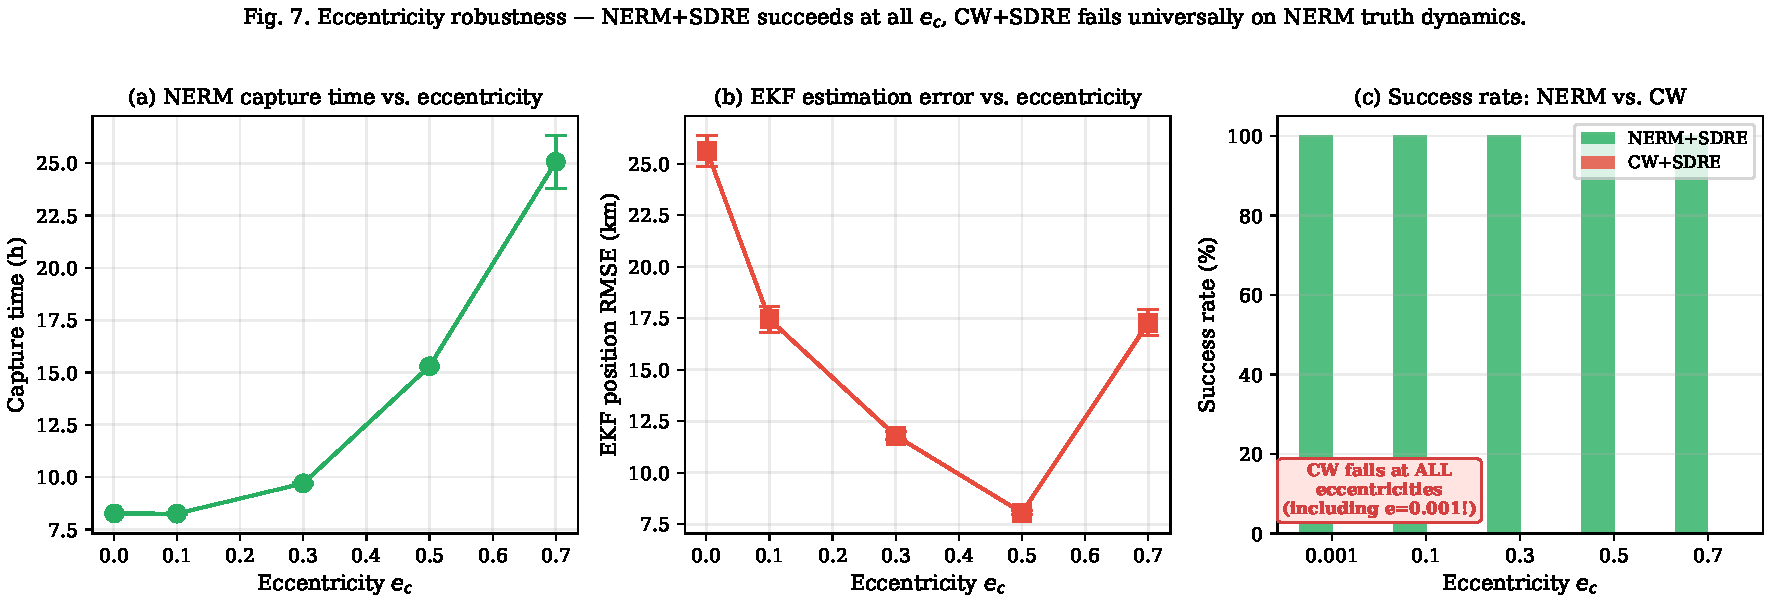
\includegraphics[width=0.95\textwidth]{fig7_eccentricity_sweep.pdf}
\caption{Eccentricity robustness analysis. (a) NERM+SDRE capture time versus $e_c$---capture succeeds at all eccentricities, with time increasing from ${\sim}29{,}800$~s at $e=0.001$ to ${\sim}87{,}300$~s at $e=0.7$. (b) EKF position RMSE versus $e_c$ (U-shaped pattern, minimum near $e=0.5$). (c) Success rate comparison: NERM+SDRE achieves 100\% at all eccentricities; CW+SDRE fails at all eccentricities including $e=0.001$ (near-circular).}
\label{fig:ecc_sweep}
\end{figure}

\subsection{Orbital Regime Sensitivity (Experiment D)}

To assess whether the common SDC-matrix framework generalizes beyond the baseline MEO scenario, we evaluated both angles-only EKF+SDRE and full-information SDRE at three orbital regimes: LEO ($a_c = 7{,}500$~km, $e_c = 0.1$, $T_{\text{orbit}} \approx 1.8$~h), MEO ($a_c = 15{,}000$~km, $e_c = 0.5$, $T_{\text{orbit}} \approx 5.1$~h, baseline), and GEO ($a_c = 42{,}164$~km, $e_c = 0.1$, $T_{\text{orbit}} \approx 23.9$~h). The initial separation is 866~km for all cases, with identical controller parameters ($Q_{\text{ctrl}} = I_6$, $R_{\text{ctrl}} = 10^{13} \cdot I_3$) and sensor noise ($\sigma_\theta = 0.008^\circ$). Five seeds are run per regime per mode.

\begin{table}[h]
\centering
\caption{Experiment D: Orbital regime comparison (5 seeds per mode per regime).}
\label{tab:expD}
\begin{tabular}{lccccc}
\toprule
Regime & $a_c$ (km) & $e_c$ & $T_{\text{orbit}}$ (h) & Mode & Success \\
\midrule
\multirow{2}{*}{LEO}  & \multirow{2}{*}{7,500}  & \multirow{2}{*}{0.1} & \multirow{2}{*}{1.8}  & Angles-only & 0/5 \\
                       &                         &                       &                        & Full-info   & 0/5 \\
\multirow{2}{*}{MEO}  & \multirow{2}{*}{15,000} & \multirow{2}{*}{0.5} & \multirow{2}{*}{5.1}  & Angles-only & \textbf{5/5} \\
                       &                         &                       &                        & Full-info   & \textbf{5/5} \\
\multirow{2}{*}{GEO}  & \multirow{2}{*}{42,164} & \multirow{2}{*}{0.1} & \multirow{2}{*}{23.9} & Angles-only & \textbf{5/5} \\
                       &                         &                       &                        & Full-info   & \textbf{5/5} \\
\bottomrule
\end{tabular}
\end{table}

\textbf{LEO: controller saturation, not filter failure.} Both angles-only and full-information modes fail to achieve the 100~m approach threshold in LEO. For the full-information SDRE, the relative distance initially expands to approximately 19,000~km due to secular along-track drift, then is reversed by the controller to a minimum of 0.37~km---within a factor of 4 of the capture threshold. However, the trajectory then rebounds to 1.3~km at the simulation end ($t = 10\,T_{\text{orbit}}$). The root cause is that the SDRE control law $u = -R^{-1} B^T P x$ scales thrust approximately linearly with distance; when $\rho < 1$~km, thrust falls below $0.6$~mm/s$^2$, which is insufficient to counteract the Coriolis acceleration $2 n v_y \sim 2$~mm/s$^2$ (with $n \approx 9.72 \times 10^{-4}$~rad/s in LEO). The fixed $R = 10^{13}$ penalty, adequate for MEO, under-powers the controller in the fast LEO dynamics. For the angles-only mode, the EKF suffers catastrophic divergence (final distance $> 3 \times 10^6$~km): the rapid LEO dynamics compress the time window for observability-enhancing geometry change, and the EKF's range estimate diverges before meaningful parallax information can be accumulated.

\textbf{GEO: capture despite large estimation error.} All five GEO trials succeed for both modes, but the angles-only EKF exhibits a pronounced stochastic bifurcation. Four of five seeds capture within 3.6--7.2~h with EKF position RMSE of $58 \pm 8$~km; the fifth seed takes 214~h to capture with an RMSE of 4,758~km and a $\Delta V$ of 4,431~km/s. The outlier is caused by near-wrapping azimuth innovations: when the EKF angular innovation approaches $\pm\pi$, the wrapping operation can introduce a $2\pi$ jump, flipping the estimated target direction by approximately $180^\circ$. In GEO's slow dynamics ($n \approx 7.29 \times 10^{-5}$~rad/s), the EKF covariance reaches steady state within a few steps and thereafter remains frozen---the Kalman gain no longer adapts to correct large estimation errors. The four normal seeds maintain moderate errors because their angular innovations never enter the wrapping-unstable region; the outlier seed enters a positive-feedback loop of wrapping-induced direction flips (83 near-wrapping events observed) that the frozen Kalman gain cannot recover from.

\textbf{The common-matrix framework has a preferred operating regime.} The MEO baseline succeeds robustly because its orbital timescale ($T \approx 5.1$~h) balances two competing requirements: (i)~sufficiently fast geometry change to provide angles-only observability through natural parallax, and (ii)~sufficiently slow dynamics to avoid Coriolis saturation of the control authority at the chosen $R$ penalty. LEO is too fast for the control budget; GEO is slow enough that the EKF covariance freezes before range becomes observable, creating a stochastic-divergence risk.

\textbf{Scope note: baseline scenario vs.\ canonical angles-only mission literature.} The baseline scenario adopted throughout this work ($\rho_0 = 866$~km, $e_c = 0.5$, MEO) sits outside the operating envelope of most published angles-only rendezvous flight-experiment work, which has demonstrated the technique at few-km to few-hundred-km separations in near-circular orbits (PRISMA and AVANTI~\cite{Gaias2014,Sullivan2017,Sullivan2021}). This scenario was chosen to \emph{stress-test} the common SDC-matrix parameterization at separations and eccentricities where linearized alternatives (CW, Tschauner--Hempel) are known to fail (§5.4)---the goal is to characterize architectural behavior at the edge of the operating envelope, not to propose a specific mission-planning tool. Extension of the framework to canonical short-range angles-only regimes is straightforward in principle (the SDC parameterization degenerates to CW as $\rho \to 0$ and $e \to 0$), but a systematic characterization at those scales is deferred to future work and would benefit from direct benchmarking against the observability-enhancing maneuver strategies of Woffinden and Geller~\cite{Woffinden2009b} and Grzymisch and Fichter~\cite{Grzymisch2014}, which are complementary to (not replaced by) the unified-matrix idea explored here.

\subsection{Discussion}

\subsubsection{Why SDC? The Case for Unified Parameterization}

The experimental results, taken together, make a cumulative argument that the SDC parameterization is a suitable modeling choice for combined estimation and control in nonlinear relative navigation---not because it produces demonstrably better closed-loop numbers than alternatives (the single-seed Ablation~A in §\ref{sec:abl_a} finds negligible differences between shared and independently evaluated $A_{\text{SDC}}$ variants), but because it provides \emph{model consistency by construction} between filter and controller and avoids the structural failures of linearized alternatives at long range.

\textbf{The SDC advantage is structural consistency, and the linearized-alternative failures are structural failures.} The identity $A(x) \cdot x \equiv f(x)$ (Eq.~\ref{eq:exact}) means the SDC factorization incurs no linearization error---it is an algebraic transformation, not a truncation. This distinguishes it from the Tschauner-Hempel (TH) equations~\cite{Tschauner1965}, which linearize the gravitational potential (though retaining elliptical-orbit periodicity), and from the CW model~\cite{Clohessy1960}, which additionally assumes a circular reference orbit. The TH model was not included as a baseline in Experiment~C because, while TH correctly captures the time-varying orbital rate $\dot{\nu}(t)$ of elliptical orbits, it shares the same linearized gravity gradient as CW---and therefore the same 80\% overestimation at 866~km separation. The TH model's failure mode would be less catastrophic than CW (the time-varying terms partially mask the gradient error) but the fundamental structural deficiency---a linear representation of a nonlinear gravitational field at large separation---persists. As demonstrated in Experiment~C (§5.4), the CW-based filter-controller pair diverges exponentially on NERM truth dynamics at \emph{all} tested eccentricities. The root cause is structural: the linear gravity gradient overestimates the true gradient by 80\% at 866~km separation, and the CW $A$-matrix lacks the nonlinear anti-damping mode (${\sim}{+}2.8 \times 10^{-4}$) present in the NERM SDC matrix. No amount of tuning can compensate for a dynamics model that structurally misrepresents the physics.

\textbf{Positioning relative to Muralidhar and Kumar (2021).} Muralidhar and Kumar~\cite{Muralidhar2021} combine an SDRE controller with a UKF estimator based on TH equations for elliptical-orbit rendezvous and docking, a configuration architecturally similar to this work but with three material differences that make a direct numerical comparison uninformative rather than clarifying. First, their filter uses TH-based dynamics with linearized gravity gradient, which as noted above breaks down at the ${\sim}$866~km separations tested here; their reported scenarios are at ${\sim}$km-range terminal rendezvous where TH is valid. Second, their controller solves a separately-parameterized ARE against a different dynamics model than the filter uses, whereas our formulation uses a single $A_{\text{SDC}}$. Third, their target-modeling assumptions (non-adversarial, small target maneuvers) differ from the zero-sum game formulation adopted here (§2.6). We therefore treat their result as complementary rather than a benchmark: they demonstrate that SDRE-based rendezvous works at canonical short range with TH dynamics; we demonstrate that a common-matrix SDC approach works at long range with full NERM dynamics. A unified benchmark on shared scenarios and shared metrics is a natural next step but requires re-implementation of their algorithm and is deferred to future work.

\textbf{Model mismatch is the hidden cost of separate architectures.} In conventional relative navigation, the EKF often employs a simplified dynamics model for computational tractability while the controller uses a higher-fidelity model for accuracy. Lee et al.~\cite{Lee2012} use an SDRE controller with an independently linearized EKF; Muralidhar and Kumar~\cite{Muralidhar2021} pair an SDRE controller with a UKF based on TH equations. In both cases, the filter predicts state evolution using different dynamics than those assumed by the controller. The unified SDC framework eliminates this mismatch: both subsystems operate on the identical $A_{\text{SDC}}(t_k)$. The numerical cost of this unification is negligible---the forward-Euler SDC discretization introduces a median per-step position error of 1.15~m (Table~\ref{tab:pred_err}), two orders of magnitude below measurement uncertainty.

\textbf{Relationship to SDRE attitude estimation-control.} Choukroun and Tekinalp~\cite{Choukroun2013} demonstrated the conceptual feasibility of using SDRE for both estimation and control in the spacecraft attitude domain. Our work extends this principle to relative position navigation and provides the explicit mechanism---the SDC exact reconstruction property---that makes the unification theoretically rigorous rather than merely convenient. Park and Kim~\cite{Park2016} validated SDREF for relative navigation but did not integrate it with control. Vepa~\cite{Vepa2018} combined estimation and control using TH equations, which---as Experiment~C demonstrates for the related CW model---do not preserve the structural fidelity of the SDC representation at medium-to-long ranges.

\subsubsection{Engineering Implications}

The inverse relationship between sensor noise and distance-threshold first-passage time (Table~\ref{tab:expB}) is empirically robust within the tested scenario, but it has limited operational meaning by itself. Across $\sigma_\theta \in [0.001^\circ, 0.1^\circ]$, the first-passage time falls by a factor of 2.3 while total $\Delta V$ remains nearly invariant and terminal relative velocity rises sharply. The single-seed Ablation~A does not support direct $A_{\text{SDC}}(\hat{\mathbf{x}})$ coupling as the dominant cause, and Ablation~C shows that the apparent benefit disappears under a velocity-constrained arrival criterion. The defensible interpretation is therefore that estimation-error-driven trajectory changes redistribute a similar control budget toward earlier sphere transit at the expense of terminal softness.

These results motivate, but do not validate, a switched guidance concept in which a long-range transfer mode is followed by an explicitly velocity-constrained terminal controller. Deliberately relaxing sensor precision is not an operational recommendation: no mode-switching simulation, field-of-view analysis, or terminal-safety guarantee is included here. Such a strategy would require independent validation against a fixed high-precision baseline using common terminal constraints, dwell-time requirements, and collision-avoidance guards.

\subsubsection{Limitations}

Several limitations bound the applicability of the present framework:
\begin{itemize}
    \item \textbf{The primary success metric is first passage, not docking.} Most reported success rates and approach times use only $\rho < 100$~m. The tightened $\rho < 100$~m and $\|\mathbf{v}_{\text{rel}}\| < 0.1$~m/s event is a soft-arrival proxy, but the simulation does not include attitude dynamics, docking-port geometry, line-of-sight keep-out constraints, contact dynamics, or a required dwell time. The results must therefore be interpreted as relative-navigation and approach performance rather than docking performance.

    \item \textbf{Mechanism attribution beyond first passage remains incomplete.} Ablation~A shows that evaluating $A_{\text{SDC}}$ at the estimate rather than the true state is negligible for one MEO baseline realization, and Ablation~C identifies the distance-only event definition as the dominant source of the apparent acceleration. However, the independent contributions of $P_0$ scaling and position- versus velocity-estimation errors have not been isolated in the 3-D model. Multi-seed, component-wise state-error interventions are required before a more specific control mechanism can be claimed.

    \item \textbf{Orbital regime specificity.} The common SDC-matrix framework with fixed control penalty $R = 10^{13}$ performs robustly in the MEO regime but fails at both extremes tested: LEO ($a_c = 7{,}500$~km, $e_c = 0.1$) and GEO ($a_c = 42{,}164$~km, $e_c = 0.1$). As demonstrated in Experiment~D (§5.5), LEO fails due to control authority saturation at close range (Coriolis forces exceeding available thrust), while GEO exhibits stochastic EKF divergence caused by angular-innovation wrapping under a frozen Kalman gain. Scheduled $Q$/$R$ matrices or regime-adaptive controller tuning would be required to extend the framework beyond MEO.

    \item The target spacecraft is assumed non-maneuvering in the nominal scenario ($\mathbf{u}_t = \mathbf{0}$). Unknown target accelerations must be absorbed by the process noise $Q$, which may be insufficient for agile targets. Extension to robust or adaptive estimation under target maneuvers remains open.

    \item At unfavorable initial geometries (large cross-track offsets combined with low initial true anomaly), the angles-only observability Gramian can become ill-conditioned. Five of 200 Monte Carlo trials (§5.3) resulted in EKF divergence. Divergence detection and recovery strategies are needed for fully autonomous operation.

    \item The single chaser-target formulation does not address multi-agent scenarios, cooperative navigation, or distributed estimation architectures.

    \item The symplectic balancing technique (§3.4) is effective for the parameter regime studied but has not been stress-tested across the full range of orbital elements and control weightings that may arise in practice.

    \item \textbf{No formal closed-loop stability guarantee; certainty-equivalence is an assumption, not a theorem.} The combined EKF+SDRE architecture constitutes a nonlinear stochastic feedback loop in which estimation error affects control, which affects the true state, which affects the next measurement. Pointwise solvability of the ARE does not guarantee closed-loop stability of the underlying nonlinear system. The SDRE control law $\mathbf{u}_c^* = -R_{\text{eff}}^{-1} B^T P \hat{\mathbf{x}}$ (Eq.~\ref{eq:uc_opt}) is a \emph{certainty-equivalence} design: it treats $\hat{\mathbf{x}}$ as if it were the true state, although classical LQG optimality conditions do not hold for this nonlinear stochastic loop. The present experiments demonstrate trajectory sensitivity to estimation error, but they do not constitute a formal proof that a separation principle fails, nor do they establish nonlinear stochastic stability. We therefore treat certainty-equivalence as a design assumption and validate behavior empirically rather than through a stability theorem.

    \item \textbf{SDC parameterization sensitivity has not been characterized.} The results reported here use the standard parameterization of Eqs.~(\ref{eq:a21})--(\ref{eq:a22}). The SDC framework is known to admit non-unique factorizations for $n > 1$~\cite{Cimen2012}, and different factorizations produce different ARE solutions and feedback laws (§2.4). Since all valid factorizations satisfy $A(\mathbf{x})\mathbf{x} \equiv f(\mathbf{x})$ exactly, perturbations to the factorization affect closed-loop behavior only through the linearization-point sensitivity of the ARE---an effect expected to diminish as estimation error converges. A systematic characterization of this sensitivity across factorizations, orbital regimes, and noise levels is deferred to future work.

    \item \textbf{Propulsion class requirements are non-trivial.} The reported peak thrust of ${\sim}1.95$~m/s$^2$ and median chaser $\Delta V$ of 8.60~km/s in Monte Carlo (Table~\ref{tab:expE}) place the required propulsion capability firmly in the bipropellant kick-stage class, well beyond the mm/s$^2$-order thrust profiles typical of monopropellant rendezvous systems. This is a direct consequence of the 866~km initial separation used in the baseline scenario and the associated $R_{\text{ctrl}} = 10^{13} I_3$ scaling that saturates peak thrust in a physically-plausible envelope. A rendezvous with mm/s$^2$-class thrust would require either shorter initial separations, longer approach horizons (increasing $R_{\text{ctrl}}$ by orders of magnitude), or a hybrid architecture using large impulsive maneuvers for the long-range transfer followed by SDRE for the terminal phase. The reader is cautioned that the numerical $\Delta V$ values reported here are architecture demonstrations at the stress-test scenario, not mission-planning recommendations.

    \item \textbf{Control-penalty $R_{\text{ctrl}}$ sensitivity is not systematically explored.} All reported results use $R_{\text{ctrl}} = 10^{13} I_3$ in km$^{-2} \cdot$s$^4$-consistent normalized units. ARE analysis predicts peak thrust scales as $\|K\| \sim 1/\sqrt{R_{\text{ctrl}}}$: reducing $R_{\text{ctrl}}$ by two orders of magnitude raises thrust toward unphysical levels, while increasing it by two orders of magnitude proportionally reduces thrust and slows approach. A full characterization of the $(R_{\text{ctrl}}, \text{approach time})$ Pareto frontier is deferred to future mission-design work.

    \item \textbf{Computational feasibility on flight hardware.} Solving a $6 \times 6$ ARE with symplectic balancing at each control step is inexpensive on a desktop-class processor (${\sim}$microseconds per solve) but has not been benchmarked on radiation-hardened flight processors (e.g., LEON3 at ${\sim}50$~MHz). The sparse update strategy ($N_{\text{are}} > 1$) mitigates this concern by reusing the cached $P$ matrix for multiple control steps, but worst-case execution time with the balancing fallback remains uncharacterized.

    \item \textbf{Practical sensor and actuator constraints.} The angles-only measurement model assumes continuous target visibility within the sensor field of view; maintaining optical lock during approach from 866~km may require attitude slews not modeled here. The SDRE controller produces continuous thrust commands, whereas real thrusters have minimum impulse bits, duty-cycle limits, and quantization effects. The interaction of thruster discretization with the common-matrix framework is not addressed.
\end{itemize}

%=====================================================================
\section{Conclusions}
%=====================================================================

This paper presented a comprehensive experimental validation of a common SDC-matrix architecture for angles-only relative navigation and SDRE optimal control of spacecraft in elliptical orbits, where a single $A_{\text{SDC}}(t_k)$ matrix simultaneously drives the EKF prediction step and the SDRE optimal control computation. The main findings are:

\begin{enumerate}
    \item \textbf{The common SDC-matrix architecture is a practical and numerically well-justified approach for combined estimation and control.} The SDC algebraic identity $A(x) \cdot x \equiv f(x)$ means the estimation and control subsystems share the same state-dependent system matrix evaluated at $\hat{x}_{k|k}$, eliminating the model mismatch that arises when they employ different dynamical representations. The forward-Euler SDC discretization introduces a median per-step position error of 1.15~m, two orders of magnitude below the angles-only measurement uncertainty (${\sim}140$~m). A known limitation of the SDC framework is that the factorization $A(x)x \equiv f(x)$ is not unique; all results reported here are conditional on the standard parameterization (Eqs.~(\ref{eq:a21})--(\ref{eq:a22})), and sensitivity to the parameterization choice remains an open question.

    \item \textbf{Distance-threshold performance is statistically reliable in MEO.} Monte Carlo analysis ($N = 200$) yields a 97.5\% threshold-reaching success rate (195/200, 95\% CI: [94.3\%, 99.1\%]) with a median first-passage time of 13.4~h and median EKF position RMSE of 12.7~km under randomized initial conditions. This statistic does not establish docking or soft-rendezvous reliability. Moreover, the framework with fixed $(Q_{\text{ctrl}}, R_{\text{ctrl}})$ parameters does not generalize across orbital regimes: LEO fails due to control authority saturation, and GEO exhibits stochastic EKF divergence from angular-innovation wrapping under a frozen Kalman gain.

    \item \textbf{Sensor noise produces a speed--softness trade-off under the distance-only approach metric.} Increasing $\sigma_\theta$ from $0.001^\circ$ to $0.1^\circ$ (100$\times$) reduces the first-passage time through the 100-m sphere by a factor of 2.3 (Spearman's $\rho = -0.89$, $p < 0.01$) while peak thrust and total $\Delta V$ remain essentially constant (${<}1\%$ variation), but terminal relative velocity increases by approximately 20$\times$. The tightened velocity-constrained criterion removes this apparent benefit for $\sigma_\theta > 0.004^\circ$, showing that faster threshold crossing is not improved soft-rendezvous performance. The single-seed Ablation~A finds negligible direct coupling through the estimated-state $A_{\text{SDC}}$ in the baseline realization. The defensible conclusion is therefore that estimation errors alter the feedback trajectory and braking history, producing earlier sphere transit at the expense of terminal softness; the separate roles of initial covariance and position/velocity estimation errors require further 3-D ablation.
\end{enumerate}

Future work includes: (i) extension to LEO and GEO regimes through scheduled $(Q_{\text{ctrl}}, R_{\text{ctrl}})$ parameter tuning; (ii) investigation of SDC parameterization sensitivity; (iii) 3-D causal ablations that independently fix $P_0$ and replace position and velocity estimates with truth channels; (iv) design and validation of a velocity-constrained terminal guidance phase with dwell-time and keep-out requirements; (v) divergence detection and recovery for the ${\sim}2.5\%$ Monte Carlo failure cases; and (vi) hardware-in-the-loop verification on space-qualified processors.

%=====================================================================
\section*{Data and Code Availability}
%=====================================================================

The closed-loop simulation framework---nonlinear elliptical relative motion (NERM) dynamics, SDC parameterization, angles-only EKF, and symplectic-balanced SDRE controller---is implemented in Python 3.12 in a project repository containing modules for dynamics (\texttt{aerospace/dynamics/nerm.py}), estimation (\texttt{aerospace/estimation/ekf.py}), control (\texttt{aerospace/control/sdre.py}), and the composed closed-loop engine (\texttt{aerospace/simulation/nerm\_ekf\_sdre.py}). Numerical results in Tables~\ref{tab:pred_err}, \ref{tab:expA}, \ref{tab:expB}, \ref{tab:expC}, \ref{tab:expD}, and \ref{tab:expE} were produced by parameter-sweep and Monte Carlo experiment scripts that call these modules; the resulting CSV output (\texttt{data/noise\_sweep\_results.csv}, \texttt{data/ecc\_sweep\_results.csv}, \texttt{data/altitude\_sweep\_results.csv}, \texttt{data/monte\_carlo\_results.csv}, \texttt{data/terminal\_vrel\_results.csv}) and the figures in this manuscript are archived alongside the code. Aggregate statistics reported in this paper (means, medians, percentiles, and standard deviations) were re-derived directly from the archived CSVs; readers seeking to reproduce or extend the analysis can regenerate any table row from the raw seed-level records. Full release of the sweep and Monte Carlo driver scripts is planned upon acceptance.

%=====================================================================
\section*{Acknowledgments}
%=====================================================================

[To be completed.]

%=====================================================================
\bibliographystyle{elsarticle-num}
\begin{thebibliography}{99}

\bibitem{Clohessy1960}
W.H. Clohessy, R.S. Wiltshire,
\newblock Terminal guidance system for satellite rendezvous,
\newblock \emph{Journal of the Aerospace Sciences}, Vol.~27, No.~9, 1960, pp.~653--658.

\bibitem{Tschauner1965}
J. Tschauner, P. Hempel,
\newblock Rendezvous zu einem in elliptischer Bahn umlaufenden Ziel [Rendezvous with a target on an elliptical orbit],
\newblock \emph{Astronautica Acta}, Vol.~11, No.~2, 1965, pp.~104--109.

\bibitem{Yamanaka2002}
K. Yamanaka, F. Ankersen,
\newblock New state transition matrix for relative motion on an arbitrary elliptical orbit,
\newblock \emph{Journal of Guidance, Control, and Dynamics}, Vol.~25, No.~1, 2002, pp.~60--66.

\bibitem{Dwidar2013}
H.R. Dwidar, A.H. Owis,
\newblock Relative motion of formation flying with elliptical reference orbit,
\newblock \emph{International Journal of Advanced Research in Artificial Intelligence}, Vol.~2, No.~6, 2013.

\bibitem{Woffinden2009}
D.C. Woffinden, D.K. Geller,
\newblock Observability criteria for angles-only navigation,
\newblock \emph{IEEE Transactions on Aerospace and Electronic Systems}, Vol.~45, No.~3, 2009, pp.~1194--1208.

\bibitem{Geller2014}
D.K. Geller, I. Klein,
\newblock Angles-only navigation state observability during orbital proximity operations,
\newblock \emph{Journal of Guidance, Control, and Dynamics}, Vol.~37, No.~6, 2014, pp.~1976--1983.

\bibitem{Gaias2014}
G. Gaias, S. D'Amico, J.-S. Ardaens,
\newblock Angles-only navigation to a noncooperative satellite using relative orbital elements,
\newblock \emph{Journal of Guidance, Control, and Dynamics}, Vol.~37, No.~2, 2014, pp.~439--451.

\bibitem{Sullivan2017}
J. Sullivan, S. D'Amico,
\newblock Nonlinear Kalman filtering for improved angles-only navigation using relative orbital elements,
\newblock \emph{Journal of Guidance, Control, and Dynamics}, Vol.~40, No.~9, 2017, pp.~2183--2200.

\bibitem{Cloutier1997}
J.R. Cloutier,
\newblock State-dependent Riccati equation techniques: an overview,
\newblock \emph{Proceedings of the American Control Conference}, 1997.

\bibitem{Cimen2010}
T. \c{C}imen,
\newblock Systematic and effective design of nonlinear feedback controllers via the state-dependent Riccati equation (SDRE) method,
\newblock \emph{Annual Reviews in Control}, Vol.~34, No.~1, 2010, pp.~32--51.

\bibitem{Cimen2012}
T. \c{C}imen,
\newblock Survey of state-dependent Riccati equation in nonlinear optimal feedback control synthesis,
\newblock \emph{Journal of Guidance, Control, and Dynamics}, Vol.~35, No.~4, 2012, pp.~1025--1047.

\bibitem{Tartaglia2016}
M. Innocenti, A. Tartaglia,
\newblock Game-theoretic strategies for spacecraft rendezvous and motion synchronization,
\newblock \emph{AIAA Guidance, Navigation, and Control Conference}, 2016. DOI: 10.2514/6.2016-0873.

\bibitem{Mracek1996}
C.P. Mracek, J.R. Cloutier, C.A. D'Souza,
\newblock A new technique for nonlinear estimation,
\newblock \emph{Proceedings of the IEEE International Conference on Control Applications}, 1996.

\bibitem{Park2016}
H.-E. Park, Y.-R. Kim,
\newblock Relative navigation for autonomous formation flying satellites using the state-dependent Riccati equation filter,
\newblock \emph{Advances in Space Research}, Vol.~57, No.~1, 2016, pp.~166--182.

\bibitem{Simhamed2021}
Y. Simhamed, F. Ykhlef, A. Iratni,
\newblock A novel frequency tracker for sinusoidal signal based on state dependent Riccati equation filter,
\newblock \emph{Measurement}, Vol.~183, 2021, 109845.

\bibitem{Vepa2018}
R. Vepa,
\newblock Application of the nonlinear Tschauner-Hempel equations to satellite relative position estimation and control,
\newblock \emph{Journal of Navigation}, Vol.~71, No.~1, 2018, pp.~44--64.

\bibitem{Okasha2011}
M. Okasha, B. Newman,
\newblock Relative motion guidance, navigation and control for autonomous orbital rendezvous,
\newblock \emph{AIAA Guidance, Navigation, and Control Conference}, 2011. DOI: 10.2514/6.2011-6427.

\bibitem{Woffinden2009b}
D.C. Woffinden, D.K. Geller,
\newblock Optimal orbital rendezvous maneuvering for angles-only navigation,
\newblock \emph{Journal of Guidance, Control, and Dynamics}, Vol.~32, No.~4, 2009, pp.~1382--1387.

\bibitem{Choukroun2013}
D. Choukroun, O. Tekinalp,
\newblock Spacecraft attitude and rate estimation and control using the SDRE method,
\newblock \emph{Proceedings of the 5th European Conference for Aeronautics and Space Sciences (EUCASS)}, Munich, 2013.

\bibitem{Lee2012}
D. Lee, J.E. Cochran, T.S. No,
\newblock Robust position and attitude control for spacecraft formation flying,
\newblock \emph{Journal of Aerospace Engineering}, Vol.~25, No.~3, 2012, pp.~436--447.

\bibitem{Muralidhar2021}
R. Muralidhar, R. Kumar,
\newblock Automated guidance and navigation for rendezvous and docking of spacecraft using SDRE controller and UKF estimator,
\newblock \emph{Proceedings of the 72nd International Astronautical Congress (IAC)}, Dubai, 2021, Paper IAC-21-C1.1.

\bibitem{Karlgaard2003}
C.D. Karlgaard, F.H. Lutze,
\newblock Second-order equations for rendezvous in a circular orbit,
\newblock \emph{Journal of Guidance, Control, and Dynamics}, Vol.~26, No.~1, 2003, pp.~41--49.

\bibitem{Sullivan2021}
J. Sullivan, S. D'Amico,
\newblock Generalized angles-only navigation architecture for autonomous distributed space systems,
\newblock \emph{Journal of Guidance, Control, and Dynamics}, Vol.~44, No.~6, 2021, pp.~1087--1105.

\bibitem{Alfriend2009}
K.T. Alfriend, S.R. Vadali, P. Gurfil, J.P. How, L.S. Breger,
\newblock \emph{Spacecraft Formation Flying: Dynamics, Control and Navigation},
\newblock Elsevier, 2009.

\bibitem{Grzymisch2014}
J. Grzymisch, W. Fichter,
\newblock Observability criteria and unobservable maneuvers for in-orbit bearings-only navigation,
\newblock \emph{Journal of Guidance, Control, and Dynamics}, Vol.~37, No.~4, 2014, pp.~1250--1260.

\end{thebibliography}

\end{document}
